% !TeX root = Documentation.tex
\documentclass[german,report,noglossaries]{hbrs-thesis}

\usepackage{blindtext}

\NewTCBListing{showcode}{ m !O{} }{
  enhanced jigsaw,
  frame hidden,
  borderline west={2pt}{0pt}{cyan},
  sharp corners,
  toptitle=0mm,
  coltitle=black,
  listing engine=minted,
  minted language=#1,
  breakable,
  minted options={linenos=false},
  colframe=cyan,
  colback=white,
  opacityback=0,
  boxrule=1pt,
  segmentation style={line width=1pt},
  grow to left by=6mm,
  grow to right by=0mm,
  left*=0mm,
  right*=0mm,
  #2
}

\NewTColorBox{showcase}{ !O{} }{
  enhanced jigsaw,
  frame hidden,
  borderline west={2pt}{0pt}{cyan},
  sharp corners,
  toptitle=0mm,
  coltitle=black,
  breakable,
  colframe=cyan,
  colback=white,
  opacityback=0,
  boxrule=1pt,
  segmentation style={line width=1pt},
  grow to left by=6mm,
  grow to right by=0mm,
  left*=0mm,
  right*=0mm,
  #1
}

\newtcolorbox{information}[1][]{%
  enhanced jigsaw, % better frame drawing
  borderline west={2pt}{0pt}{cyan}, % straight vertical line at the left edge
  sharp corners, % No rounded corners
  boxrule=0pt, % no real frame,
  fonttitle={\bfseries},
  coltitle={black},  % Black colour for title
  title={Information: \ },  % Fixed title
  attach title to upper, % Move the title into the box
  #1
}

\begin{document}
\begin{titlepage}
    \begin{center}
        {\LARGE Dokumentation zu \texttt{hbrs-thesis}}
        \vfill
        {\Huge \textit{Modern und einfach}}
        \vfill
        {\LARGE Version 1.0}\\
        \vspace{2em}
        {\Large \today}
    \end{center}
\end{titlepage}

\tableofcontents
\listoffigures
\listofcode

\chapter{Vorwort}
Diese Dokumentation ist nicht vollumfänglich. Das bedeutet, dass sie nicht auf alle Eigenheiten der einzelnen verwendeten Pakete eingeht. Für weitere und aktuelle Informationen empfehle ich immer die Recherche auf \url{https://www.ctan.org/}, wo alle Pakete mit ihren Dokumentationen hinterlegt sind.

In diesem Dokument werden die wichtigsten Befehle gezeigt und erklärt. Diese Dokumentation kann und sollte gerne durch die Hilfe der Community korrigiert und erweitert werden.

Viel Erfolg beim Schreiben!
\chapter{Verwendung der \LaTeX-Klasse}
Um die Klasse als Vorlage für Dokumente zu verwenden, empfiehlt es sich, den kompletten Ordner \texttt{template} zu kopieren und entsprechend dieser Dokumentation zu verwenden. In diesem Kapitel werden die einzelnen Bestandteile des Ordners kurz erklärt. Die Verwendung der einzelnen Ordner und Dateien wird im späteren Verlauf des Dokuments näher erläutert.

\section{Bestandteile des Templates}
Die Konfiguration aller Informationen auf dem Deckblatt, sowie die Widmung können \marginpar{\texttt{assets/\\utility/*}}über die Datei \texttt{assets/utility/meta.tex} angepasst werden. Innerhalb des Ordners \texttt{assets/utility} finden sich außerdem noch eine Datei für Worttrennungen, die von \LaTeX nicht korrekt erkannt werden (\texttt{hyphenation.tex}), Akronyme (\texttt{acronyms.tex}) und Glossareinträge (\texttt{glossary.tex}).

In \texttt{assets/images} werden Bilder hinterlegt. Je nach Anzahl der Bilder im Dokument \marginpar{\texttt{assets/\\images/*}}empfiehlt es sich, diese nach Kapitel zu sortieren. Im Ordner \texttt{assets/images} befindet sich bereits ein Ordner \texttt{titlepage}, welcher die Bilder für die Titelseite enthält. Diese sollten nicht gelöscht werden, da sonst die Titelseite und somit das Dokument nicht mehr gebaut werden kann.

Der Ordner \texttt{chapter} ist dafür gedacht, die Kapitel oder Abschnitte (je nach Verwendung der Dokumentklasse (siehe \autoref{chap:klassenoptionen})) \marginpar{\texttt{chapter}}aufzuteilen und die entsprechenden Dateien dort abzulegen. Diese Aufteilung bringt den Vorteil, dass Kapitel sehr schnell neu sortiert werden können. Zusätzlich enthalten die Dateien weniger Text und sind damit übersichtlicher.

Zu einem wissenschaftlichen Dokument gehört auch Literatur. Die Informationen zu dieser \marginpar{\texttt{biblio-\\graphy.bib}}Literatur werden als BibTeX oder BibLaTeX in der Datei \texttt{bibliography.bib} hinterlegt. Ich persönlich bevorzuge es die PDF-Dokumente lokal mit abzuspeichern. Mit lokalen Dateien habe ich die Möglichkeit Anmerkungen zu machen und die Dateien mit anderer Software besser zu durchsuchen (siehe \url{https://github.com/freedmand/semantra}). Die PDF-Dokumente kommen dann in den dieser \marginpar{\texttt{literature}}Ordner \texttt{literature}. Je nach Literaturverwaltungssoftware können Einstellungen getroffen werden, um diese Dokumente direkt in der Software aufzurufen.

Für den Bau des Dokuments mit \texttt{latexmk} wird die Datei \texttt{.latexmkrc} benötigt, da sie \marginpar{\texttt{.latexmkrc}}Informationen zum Bauen des Dokumentes mit Glossar und Akronymen enthält. Wird kein Glossar- und/oder Akronymverzeichnis benötigt, empfiehlt es sich, die entsprechende Option in der Klasse zu verwenden (siehe \autoref{chap:klassenoptionen}).

Beim Kompilieren des Dokumentes entsteht ein neuer Ordner \texttt{out}. \marginpar{\texttt{out}}Dieser Ordner enthält verschiedene Kompilierungsschritte, Log- und Synchronisierungsdateien von \LaTeX. Im Zweifel kann dieser Ordner gelöscht und der Buildprozess neu gestartet werden. Die darin befindliche PDF-Datei (das gebaute Dokument) sollte jedoch vorher gespeichert werden, um einen Verlust der Daten zu vermeiden. Vorschläge für eine Konfiguration von \LaTeX-Umgebungen in verschiedenen IDEs werden auch noch vervollständigt.

Zuletzt befindet sich in \texttt{hbrs-thesis.cls} sämtliche Konfiguration für die Klassendatei. \marginpar{\texttt{hbrs-\\thesis.cls}}Diese Konfiguration kann nach Belieben angepasst werden. Sollten Grundsätzliche Änderungs- oder Verbesserungsvorschläge an dieser Datei entstehen, bitte ich darum, diese auch bei GitHub (siehe \url{https://github.com/blackapple113/H-BRS-Thesisvorlage}) einzureichen.
\chapter{Optionen der Klasse hbrs-thesis}
\label{chap:klassenoptionen}
Für die Modularität der Klasse wurden einige Optionen eingebaut. Mithilfe dieser Optionen lässt sich das Dokument zum Teil in Optik und Verwendungszweck anpassen. Im Folgenden werden die Optionen mit Beispielen erläutert.

\section{Spracheinstellungen}
Eine Pflichtoption, welche für eine korrekte Worttrennung verwendet werden muss ist die Einstellung der Sprache. Die Sprache kann aktuell nur zwischen englisch und deutsch unterschieden werden. Weitere Anpassungsmöglichkeiten für komplexere bilinguale Dokumente oder andere Spracheinstellungen müssen über die Datei \texttt{hbrs-thesis.cls} manuell eingestellt werden. Angenommen es wird ein Dokument auf Deutsch geschrieben, so muss in Kombination mit dieser Klasse die Option auf \texttt{german} gesetzt werden. Intern werden dann Optionen für die Deutsche Sprache gesetzt. Wird das Dokument auf Englisch geschrieben, so muss \texttt{english} angegeben werden. 

\begin{code}{latex}
\documentclass[german]{hbrs-thesis}
…
\end{code}

Werden bilinguale Spracheinstellungen im Dokument benötigt, müssen in der Klassendatei \texttt{hbrs-thesis.cls} Einstellungen für das Paket \texttt{babel} getroffen werden. Das Paket befindet sich unter der Region \texttt{Required packages}. Ist die Hauptsprache des Dokuments Englisch, kommen aber durchaus Deutsche Begriffe darin vor, eignet sich die Konfiguration \mintinline{latex}{\RequirePackage[ngerman,english]{babel}}. Die zuletzt angegebene Sprache ist die Hauptsprache.

\begin{information}
    Wird die Sprache über die Optionsmöglichkeiten für das Paket \texttt{babel} direkt in \texttt{hbrs-template.cls} geändert, dürfen keine Sprachangaben als Klassenoptionen gesetzt werden.
\end{information}

\section{Stiloptionen}
Die Klasse besitzt ein paar Optionen, um verschiedene Stile anzubieten. Mithilfe der Option \texttt{classicstyle} bzw. \texttt{modernstyle} kann zwischen einer Schriftart mit Serifen und einer serifenlosen Schriftart (was sind Serifen: \url{https://de.wikipedia.org/wiki/Serife}) unterschieden werden. Serifen sollen dem Lesenden helfen die Zeilen besser zu verfolgen, um während des Lesens nicht in der Zeile zu verrutschen, sind aber auf Bildschirmen teilweise schlechter darzustellen. Der Standard ist hier \texttt{modernstyle} und muss somit nicht explizit angegeben.
\begin{showcase}
\begin{code}{latex}
\documentclass[german,classicstyle]{hbrs-thesis}
…
\end{code}
\tcblower
\begin{figure}[H]
    \centering
    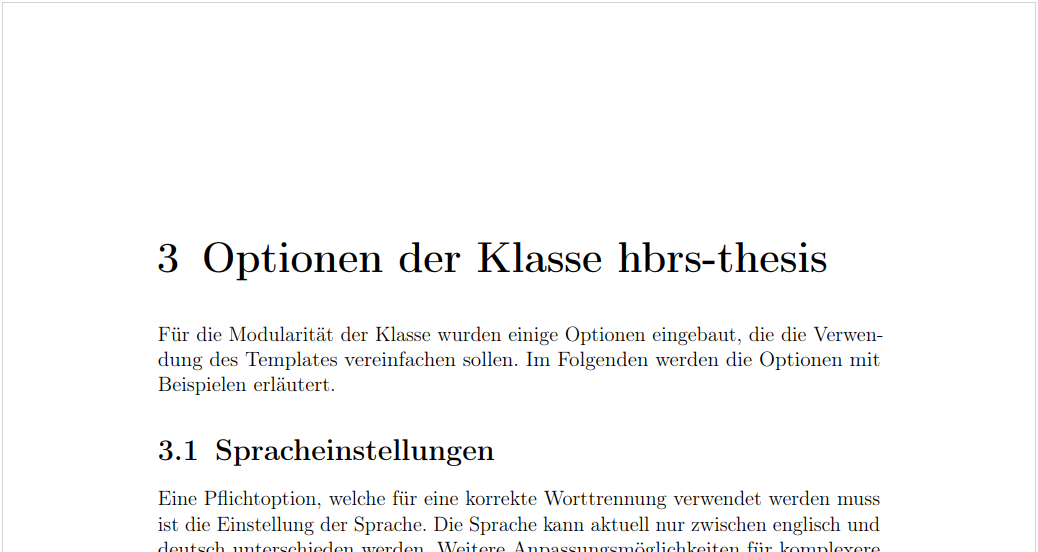
\includegraphics[width=0.8\columnwidth]{assets/images/klassenoptionen/classicstyle.png}
    \caption{Beispielbild für die Option \texttt{classicstyle}.}
\end{figure}
\end{showcase}

Neben dem Stil der Schriftart kann auch zwischen \texttt{report} und \texttt{article} unterschieden werden. Report bietet einzelne Kapitel beschrieben durch \mintinline{latex}{\chapter{…}} welche immer auf einer neuen Seite anfangen. Im Gegensatz dazu bietet \texttt{article} lediglich Abschnitte beschrieben durch \mintinline{latex}{\section{…}}, die nicht jedes Mal auf einer neuen Seite beginnen. Diese beiden Stile können durch die Größe des entstehenden Dokumentes unterschieden werden. Zum Beispiel wird so bei einem Praxisprojektbericht \texttt{article} verwendet wohingegen für eine Thesis \texttt{report} geeignet erscheint. Da die Dokumente nicht doppelseitig ausgedruckt werden entfällt die Option für ein Buchlayout. Diese wird vielleicht später noch hinzugefügt. \textbf{Die Option \texttt{article} ist standardmäßig konfiguriert.} Für eine Thesis sollten die Optionen für die Klasse \texttt{hbrs-thesis} also z.\,B. wie folgt verwendet werden:

\begin{code}{latex}
\documentclass[german,classicstyle,report]{hbrs-thesis}
…
\end{code}

\section{Druckoptionen}
Soll das Dokument ausgedruckt und gebunden werden ergibt sich die Notwendigkeit für einen erweiterten Seitenrand an der Bindeposition (innerer Seitenrand). Mit der Option \texttt{noprint} kann im Dokument explizit angegeben, dass dieses Dokument nicht gedruckt und gebunden wird. So verschiebt sich der Textbereich mittig auf die Seite mit gleichmäßigen Seitenrändern. Standardmäßig ist die \texttt{noprint} Option deaktiviert, da es sich bei der Vorlage um eine Thesisvorlage handelt und diese in der Regel ausgedruckt wird.

\begin{code}{latex}
\documentclass[german,noprint]{hbrs-thesis}
…
\end{code}

\section{Glossar und Akronymverzeichnis}
Werden kein Glossar und/oder Akronymverzeichnis verwendet empfiehlt es sich die Option \texttt{noglossaries} in der Klasse zu verwenden. Damit wird das entsprechende Paket nicht geladen, es wird keine Warnung diesbezüglich ausgegeben und das Kompilieren geht eventuell schneller.

\begin{code}{latex}
\documentclass[german,noglossaries]{hbrs-thesis}
…
\end{code}

\section{Aus PDF kopieren}
Für die bessere Unterstützung des heraus Kopierens von Text aus der fertigen PDF-Datei wird das Paket \texttt{mmap} verwendet. Aufgrund der Einstellungen der Schriftart werden jedoch sehr viele Warnungen ausgegeben, weshalb die Option standardmäßig deaktiviert ist. Um den Lesenden ein einfacheres Kopieren von Inhalten zu ermöglichen, kann das Paket \texttt{mmap} mit der gleichnamigen Option aktiviert werden.

\begin{code}{latex}
\documentclass[german,mmap]{hbrs-thesis}
…
\end{code}
\chapter{Generelles}

\section{Referenzen}
\label{sec:referenzen}
\begin{wraptable}{r}{0.4\textwidth}
    \vspace{-2em}
    \captionabove{Präfixe für Referenzen}
    \centering
    \begin{tblr}{ll}
        \toprule
        \textbf{Prefix} & \textbf{Bezeichnung} \\
        \midrule
        ch: & chapter \\
        sec: & section \\
        subsec: & subsection \\
        fig: & figure \\
        subfig: & sub figure \\
        tab: & table \\
        subtab: & sub table \\
        eq: & equation \\
        code: & code listing \\
        itm: & enumerated list item \\
        alg: & algorithm \\
        app: & Anhang \\
        \bottomrule
    \end{tblr}
    \label{tab:praefixe-fuer-referenzen}
\end{wraptable}

Die Funktion \mintinline{latex}{\label{}} in \LaTeX dient dazu, Markierungen innerhalb des Textes zu setzen, auf die später mithilfe von Referenzen zugegriffen werden kann. Dies ist besonders nützlich, um Verweise auf Abschnitte, Kapitel, Gleichungen, Abbildungen oder Tabellen innerhalb eines \LaTeX-Dokuments zu erstellen. Label sollten für die einfachere Zuordnung aussagekräftig beschrieben sein. So bietet es sich zum Beispiel an für Kapitel (engl. chapter) \texttt{ch:} an den Anfang des Labels zu schreiben, für Abschnitte (engl. section) \texttt{sec:}, usw (vgl. \autoref{tab:praefixe-fuer-referenzen}). Indem man ein Label mit einem eindeutigen Namen an der gewünschten Stelle platziert, kann man später im Text mithilfe von \mintinline{latex}{\autoref{}} auf dieses Label verweisen, um automatisch die Bezeichnung inkl. Nummer einzufügen. Dies erleichtert die Aktualisierung von Referenzen, wenn sich die Nummerierung oder Anordnung im Dokument ändert, da LaTeX automatisch die korrekten Nummern aktualisiert.

\begin{showcode}{latex}
    \subsection{Beispiel für Referenzen}
    \label{subsec:beispiel-fuer-referenzen}

    Wie in \autoref{subsec:beispiel-fuer-referenzen} beschrieben…
\end{showcode}

Bei der Vergabe eindeutiger Bezeichner für die Referenzierung sollte darauf geachtet werden, dass lediglich ASCII-Zeichen verwendet werden. Je nach Kodierung der Quelldatei können Sonderzeichen sonst zu Fehlermeldungen führen. Sollten Teilelemente (sub figure, sub table) referenziert werden existieren zwei Möglichkeiten. Angenommen man benennt ein Teilelement mit \mintinline{latex}{\label{subfig:testbild}}, kann mit \mintinline{latex}{\autoref{sub@subfig:testbild}} allein auf die Nummerierung des Teilelements verwiesen werden, wohingegen mit \mintinline{latex}{\autoref{subfig:testbild}} die Abbildungsnummer der übergeordneten Beschriftung vorangestellt wird. Beispiele und näheres dazu in \autoref{chap:bilder}.

\subsection{Weitere Referenzmöglichkeiten}

\begin{description}
    \item[\mintinline{latex}{\label{}}] Gibt dem zu referenzierenden Objekt einen Namen, auf den später referenziert werden kann.
    \item[\mintinline{latex}{\ref{}}] Referenziert auf das Objekt und gibt nur die Nummer für dieses Objekt zurück (sollte nur selten verwendet werden).
    \item[\mintinline{latex}{\pageref{}}] Gibt die Seitenzahl des referenzierten Objektes zurück.
    \item[\mintinline{latex}{\autoref{}}]\label{itm:autoref} Referenziert auf das Objekt mit der Bezeichnung und der Nummer. \textbf{Dies ist die präferierte Variante.}
    \item[\mintinline{latex}{\nameref{}}] Gibt den Inhalt des naheliegendsten relevanten Objekt zurück. So wird bei einer Überschrift diese zurückgegeben, aber für ein Bild der Inhalt der Bildunterschrift.
\end{description}

\section{Fließumgebungen}
\label{sec:fliessumgebungen}
Fließumgebungen (engl. floats) sind ein wichtiger Bestandteil von \LaTeX-Dokumenten, um Grafiken, Abbildungen, Tabellen und ähnliche Inhalte flexibel und ästhetisch ansprechend im Layout zu platzieren. Durch die Verwendung von Fließumgebungen können diese Elemente automatisch an geeigneten Stellen im Text platziert werden, um den Lesefluss nicht zu unterbrechen. Innerhalb von Fließumgebungen kann der Befehl \mintinline{latex}{\caption{}} verwendet werden, um Bild- oder Tabellenbeschriftungen hinzuzufügen, sowie der Befehl \mintinline{latex}{\label} (siehe \autoref{sec:referenzen}), um Labels für Referenzen festzulegen. 

Trotz der automatischen Platzierung von Fließumgebungen in \LaTeX gibt es Situationen, in denen eine manuelle Kontrolle über die Positionierung erforderlich ist. \LaTeX bietet Optionen, um Fließumgebungen an bestimmten Stellen im Text zu platzieren. Die Option \texttt{[h]} (here) erlaubt eine Platzierung am Ort des Befehls im Text. \texttt{[t]} (top) platziert die Umgebung oben auf einer Seite, \texttt{[b]} (bottom) unten auf einer Seite und \texttt{[p]} (page) auf einer separaten Seite nur für Fließumgebungen. Soll die Fließumgebung fix an die vom Autor angegebene Stelle platziert werden, kann die Option \texttt{[H]} (Here!) verwendet werden. Diese Option zwingt \LaTeX zur Positionierung an der angegebenen Stelle. Manuelle Positionierungsoptionen sollten jedoch sparsam verwendet werden, da sie die typografische Ästhetik beeinträchtigen könnten.

\subsection{Beschriftungen}
\label{sec:beschriftungen}
In \LaTeX ermöglicht der Befehl \mintinline{latex}{\caption{}} das Hinzufügen von Beschriftungen zu Fließumgebungen. Diese Beschriftungen bieten eine kurze Erklärung oder Bezeichnung für das jeweilige Element. Beschriftungen sind hilfreich, um den Inhalt für den Leser zu erläutern und in den Kontext des Dokuments zu setzen. Darüber hinaus generiert \LaTeX automatisch die richtige Nummerierung für Abbildungen und Tabellen, was die Konsistenz und Verwaltung erleichtert. Durch die Kombination von \mintinline{latex}{\caption{}} mit \mintinline{latex}{\label{}} können Sie außerdem Referenzen zu diesen Elementen erstellen, die im Text automatisch die korrekte Nummer und Bezeichnung anzeigen (vgl. \autoref{itm:autoref}). Mit dem Befehl \mintinline{latex}{\captionof{float}{}} können Beschriftungen auch außerhalb von Fließumgebungen für bestimmte Elemente gesetzt werden. 

Für Tabellen werden in wissenschaftlichen Artikeln die Beschriftungen häufig oberhalb des Elements gesetzt, da die Beschriftung unterhalb der Tabelle bei langen Tabellen zu spät gelesen wird. Bei Bildern hingegen sind die Beschriftungen unterhalb des Elements. Da die Formatierung von \LaTeX diesen Unterschied bei Tabellen nicht berücksichtigt existiert in diesem Dokument der Befehl \mintinline{latex}{\captionabove{}}, welcher den Abstand zwischen Beschriftung und Tabelle korrigiert.

Werden mehrere Tabellen oder Bilder in einer Fließumgebung nebeneinander gezeigt sollten auch die Teilelemente einzelne Beschriftungen bekommen. Diese können mit dem Befehl \mintinline{latex}{\subcaption{}} erstellt werden.

\subsection{Zentrierung}
Es ist oft sinnvoll, Fließumgebungen wie Tabellen oder Bilder zu zentrieren, insbesondere wenn sie nicht die volle Textbreite ausfüllen. Dies trägt zur ästhetischen Gestaltung des Dokuments bei und sorgt dafür, dass diese Elemente optisch ausgerichtet und präsentiert werden. Es gibt zwei gängige Möglichkeiten, dies in \LaTeX zu erreichen.

Die erste Möglichkeit ist die Verwendung der \texttt{center}-Umgebung, welche \textbf{keine} Fließumgebung darstellt:

\begin{showcode}{latex}
    \begin{center}
        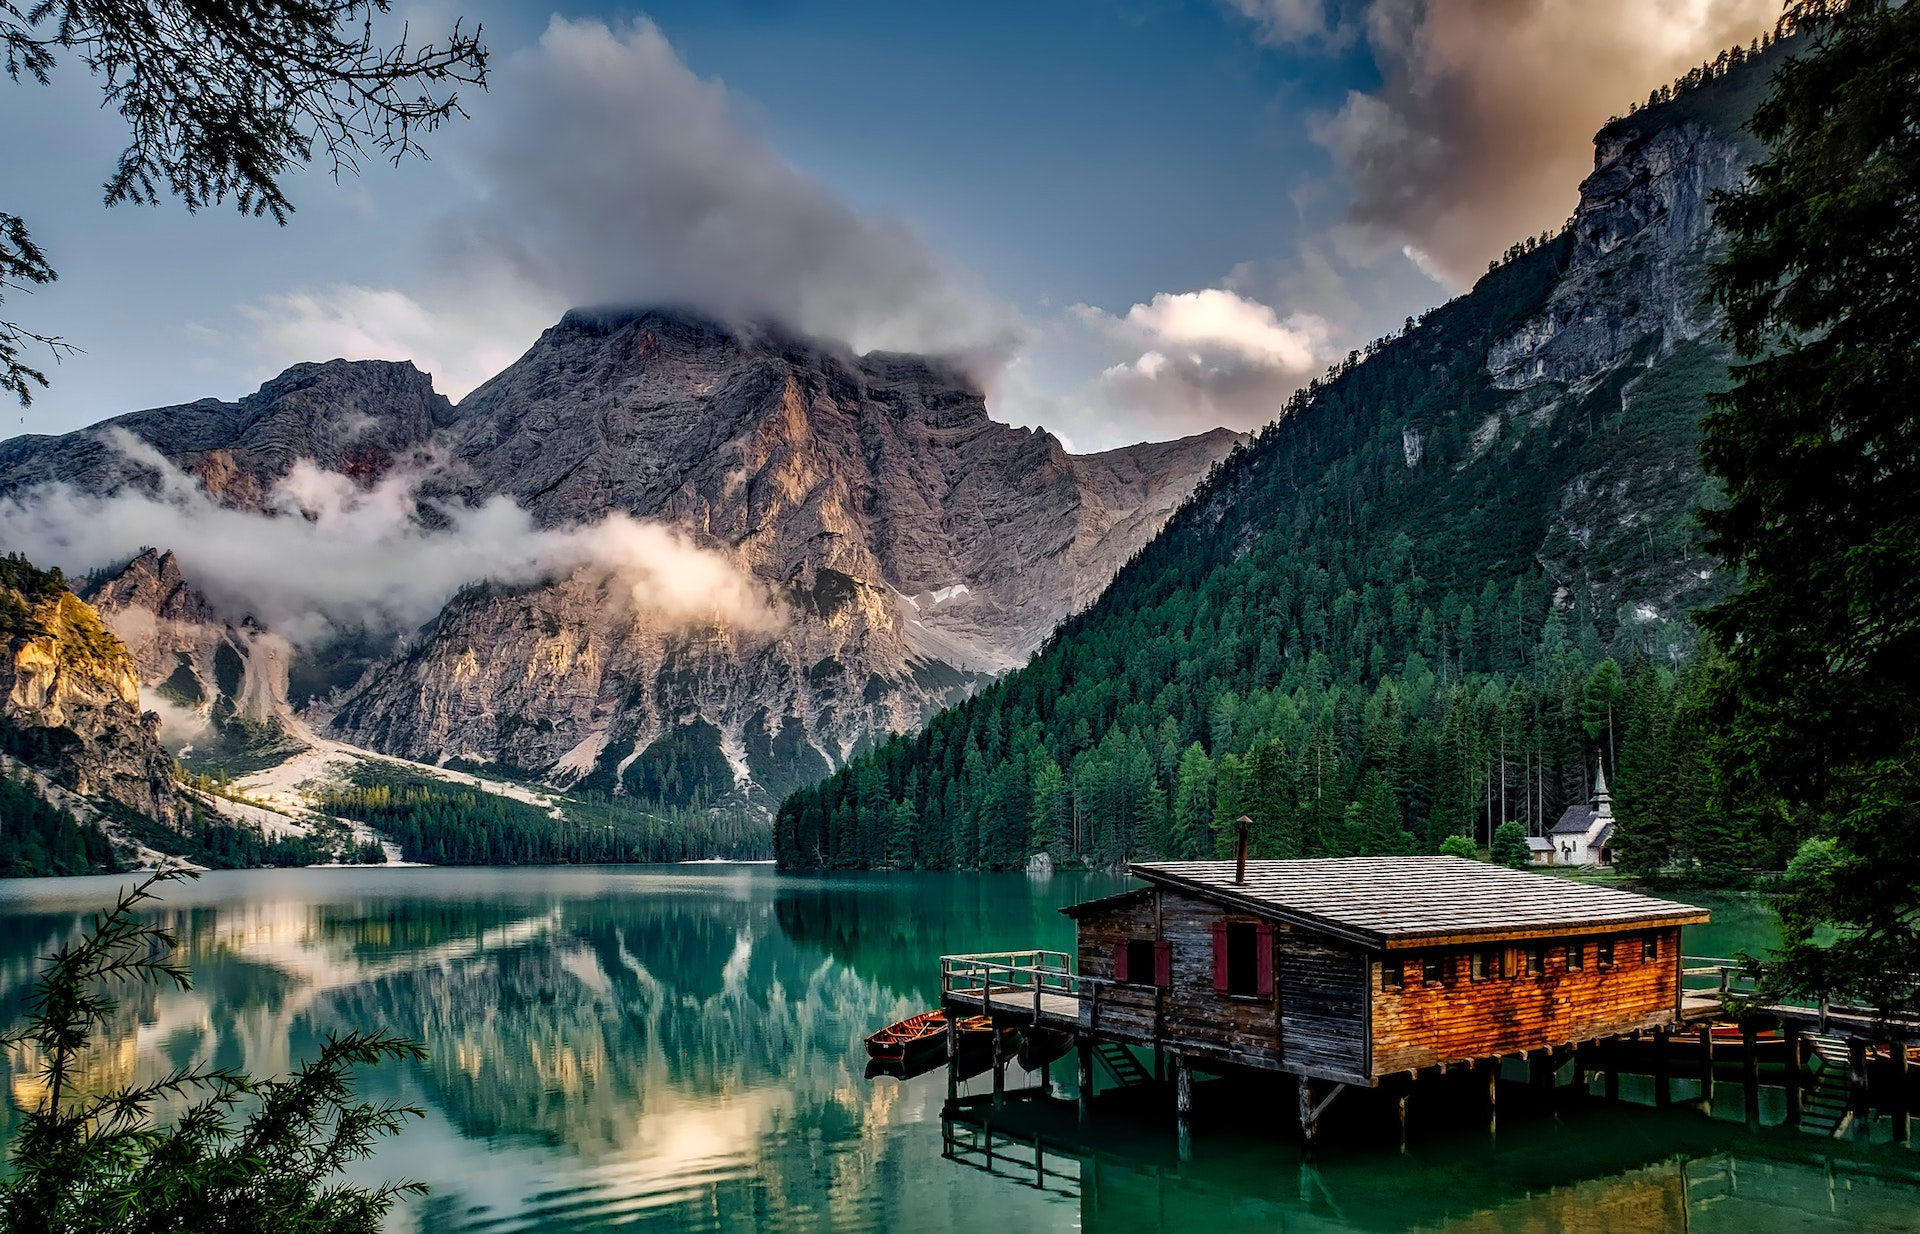
\includegraphics[width=0.4\columnwidth]{assets/images/bilder/pexels-pixabay-147411.jpg}
        \captionof{figure}{Beschriftung des Bildes}
    \end{center}
\end{showcode}

Die zweite Möglichkeit ist die Verwendung des Befehls \mintinline{latex}{\centering} innerhalb einer Fließumgebung:

\begin{showcase}
    \begin{code}{latex}
        \begin{figure}
            \centering
            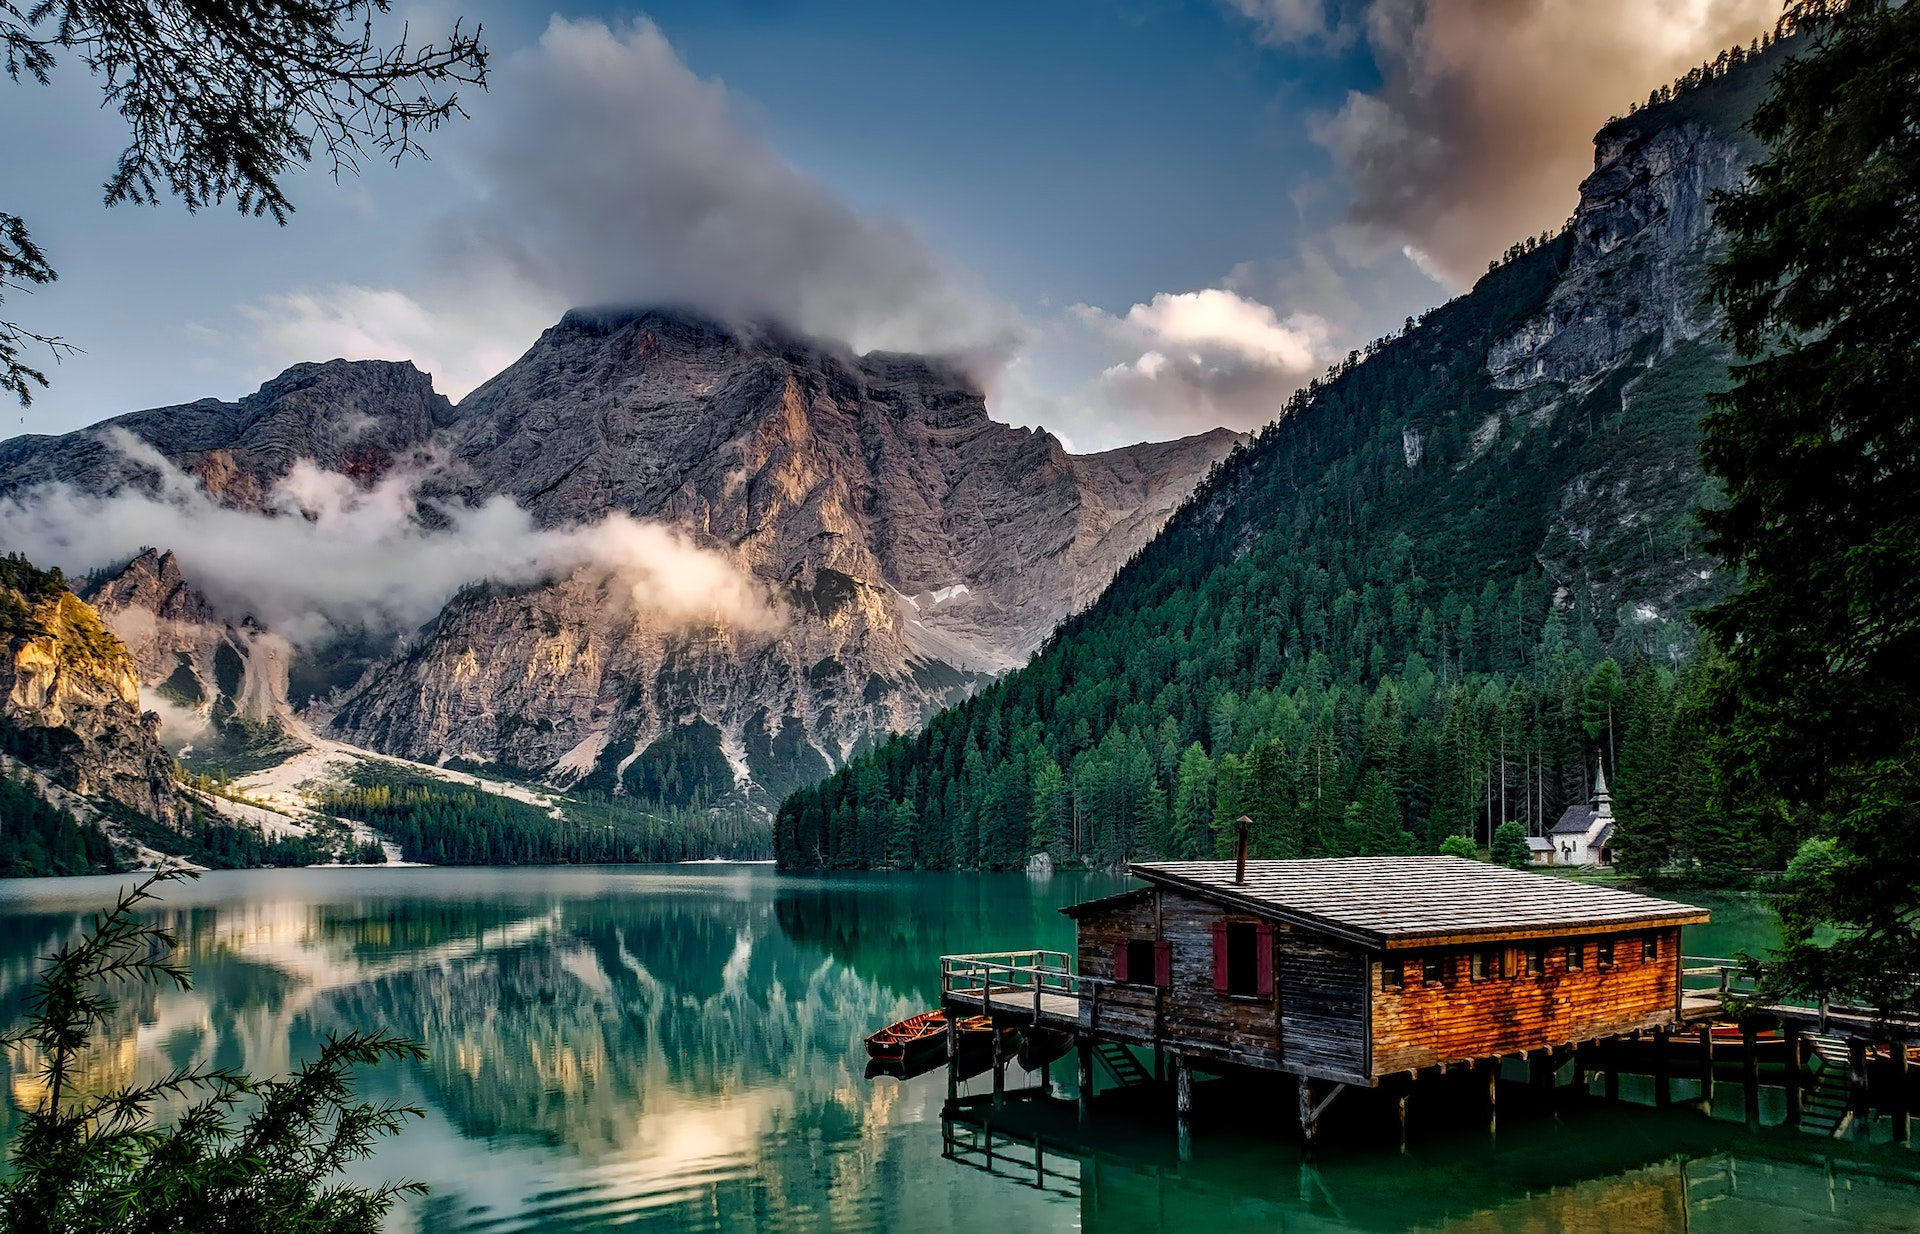
\includegraphics[width=0.4\columnwidth]{assets/images/bilder/pexels-pixabay-147411.jpg}
            \caption{Beschriftung des Bildes}
        \end{figure}
    \end{code}
    \tcblower
    \begin{center}
        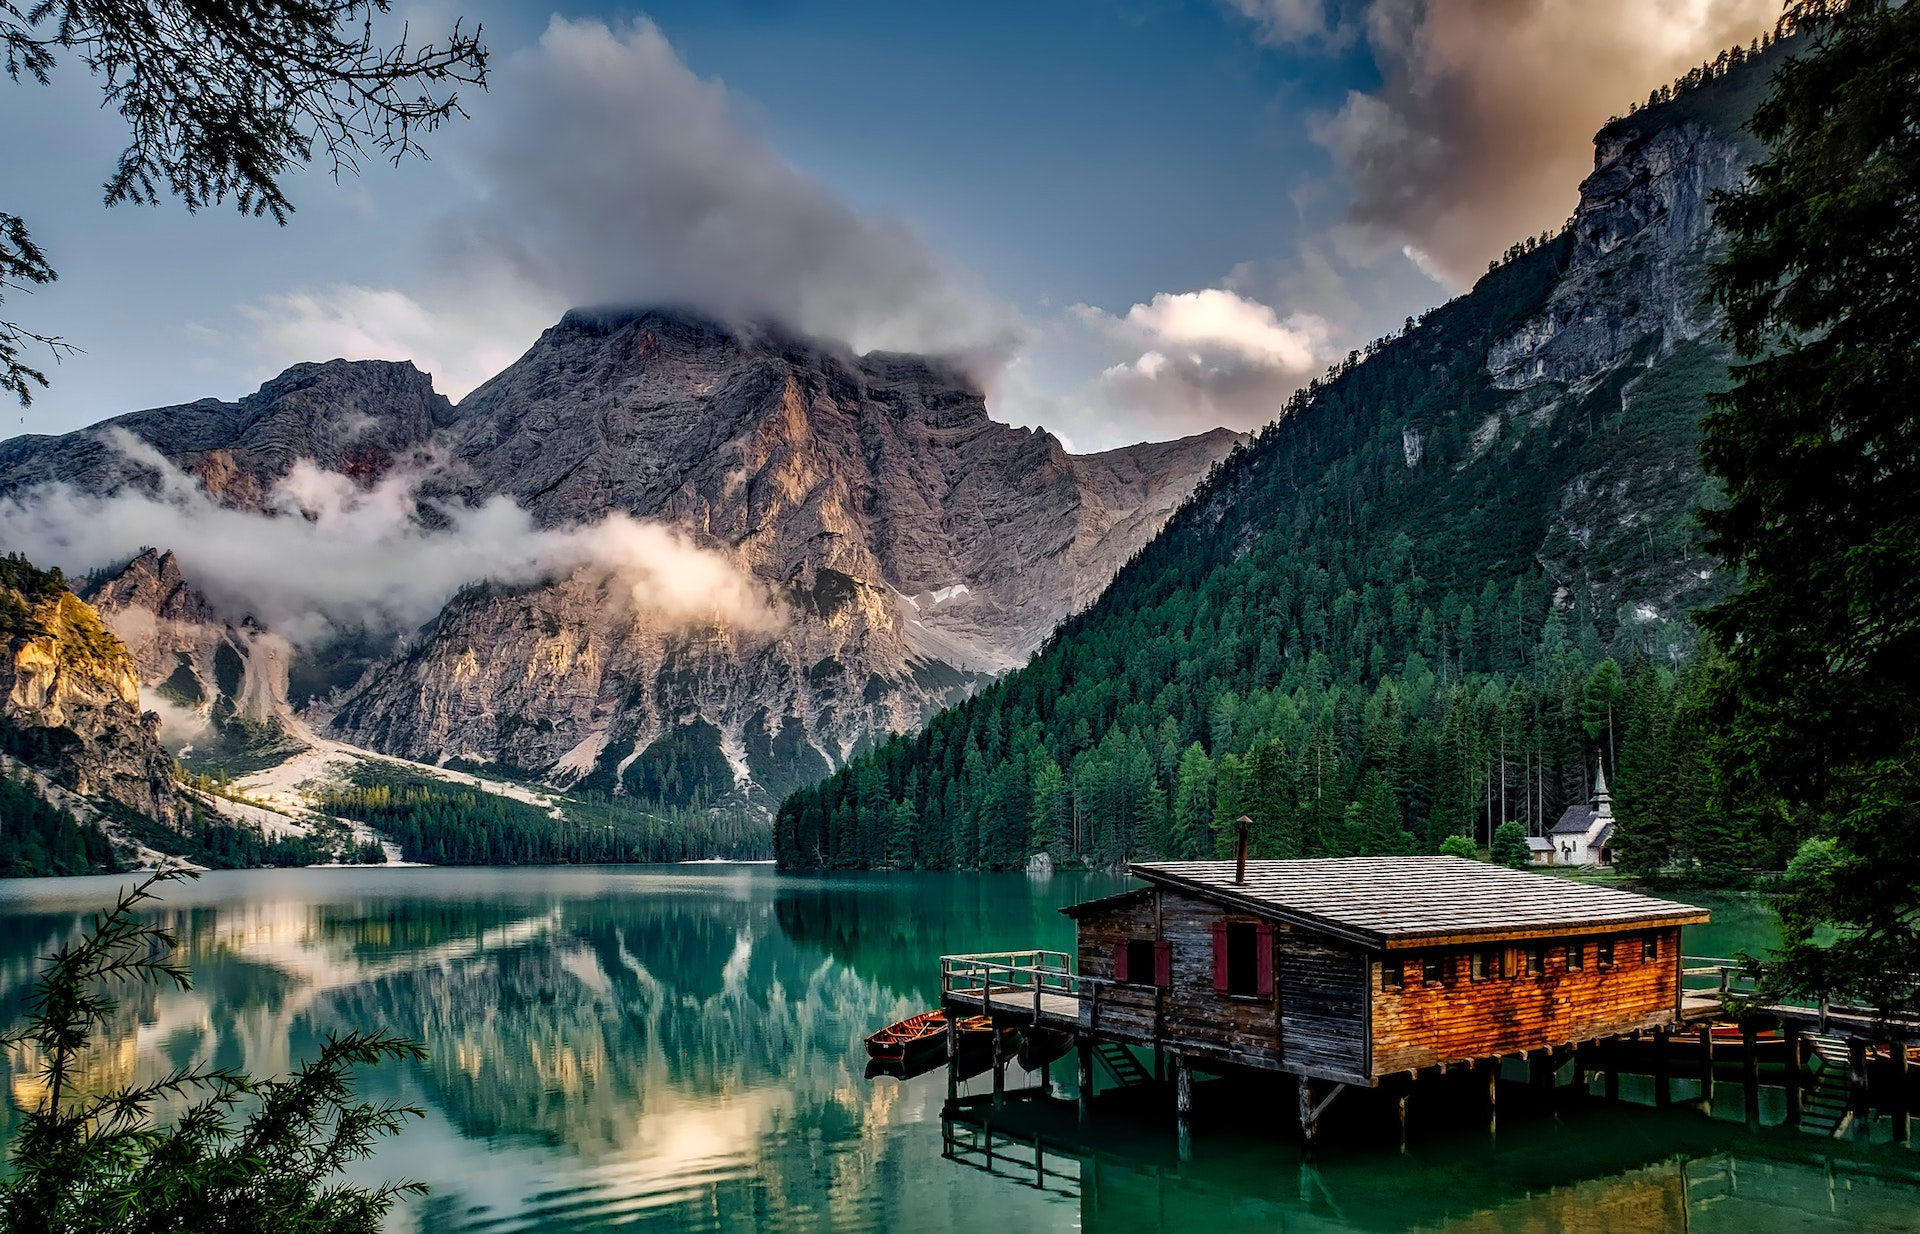
\includegraphics[width=0.4\columnwidth]{assets/images/bilder/pexels-pixabay-147411.jpg}
        \captionof{figure}{Beschriftung des Bildes}
    \end{center}
\end{showcase}

Beide Methoden zentrieren den Inhalt horizontal im Dokument. Mit der \texttt{center}-Umgebung erhalten wir jedoch keine Fließumgebung, weshalb wir für eine Beschriftung des Bildes den Befehl \mintinline{latex}{\captionof{figure}{}} verwenden müssen. Wie in \autoref{sec:fliessumgebungen} beschrieben ist auch keine optimierte Positionierung des Elements durch \LaTeX möglich.

\section{Minipage}
\label{sec:minipage}
Mit der Umgebung \texttt{minipage} können in \LaTeX Elemente wie Bilder, Tabellen aber auch Texte in ihrer Größe begrenzt und nebeneinander platziert werden. Eine \texttt{minipage}-Umgebung wird wie folgt definiert:

\begin{code}{latex}
    \begin{minipage}[outer position][height][inner pos]{width}
        % Inhalt
    \end{minipage}
\end{code}

\begin{description}
    \item[\mintinline{latex}{width}] Die Breite ist eine Pflichtangabe und beschreibt, wie breit die \texttt{minipage} sein soll. Hierbei empfehlen sich angaben wie bei Bildern mit \mintinline{latex}{\columnwidth}, \mintinline{latex}{\textwidth} oder \mintinline{latex}{\linewidth}.
    \item[\mintinline{latex}{outer position}] Gibt an, wie die \texttt{minibox} ausgerichtet werden soll.
    \item[\mintinline{latex}{height}] Die Größe der \texttt{minibox} ist dynamisch an den Inhalt angepasst. Mit dieser Angabe kann die Höhe der Box verändert werden.
    \item[\mintinline{latex}{inner pos}] Gibt die vertikale Positionierung des Textes innerhalb der Box an, wenn die Box größer ist, als der Text.
\end{description}

\subsection{Äusere Positionierung (outer position)}
\begin{showcode}{latex}
    Grundlinie
    \begin{minipage}[b]{0.17\linewidth}
        \textbf{Eine \texttt{minipage} unten ausgerichtet.}
    \end{minipage}
    ------------
    \begin{minipage}{0.17\linewidth}
        \textbf{Eine \texttt{minipage} mittig ausgerichtet.}
    \end{minipage}
    ------------
    \begin{minipage}[t]{0.17\linewidth}
        \textbf{Eine \texttt{minipage} oben ausgerichtet.}
    \end{minipage}
    Grundlinie
\end{showcode}

\subsection{Innere Positionierung (inner position)}
\begin{showcode}{latex}
    Grundlinie
    \begin{minipage}[b][3cm][t]{0.17\linewidth}
        \textbf{Ein Paragraph oben ausgerichtet.}
    \end{minipage}
    ------------
    \begin{minipage}[b][3cm][c]{0.17\linewidth}
        \textbf{Ein Paragraph mittig ausgerichtet.}
    \end{minipage}
    ------------
    \begin{minipage}[b][3cm][b]{0.17\linewidth}
        \textbf{Ein Paragraph unten ausgerichtet.}
    \end{minipage}
    Grundlinie
\end{showcode}
\chapter{Bilder}
\label{chap:bilder}
Für qualitativ hochwertige Dokumente sollten möglichst hochauflösende Bilder oder SVG-Grafiken (\url{https://de.wikipedia.org/wiki/Scalable_Vector_Graphics}) verwendet werden, da besonders im Druck schlechte Auflösungen negativ hervorstechen.

Bilder können in die \textit{Fließumgebung} \texttt{figure} gepackt werden. Für Positionierungsoptionen siehe \autoref{sec:fliessumgebungen}. Das Bild innerhalb der Fließumgebung \texttt{figure} wird mit dem Befehl \mintinline{latex}{\includegraphics[options]{path}} durch das Paket \texttt{graphicx} eingefügt. In \texttt{options} sollte immer die Option \mintinline{latex}{width=\columnwidth} gesetzt werden. Bei einem einspaltigen Layout kann alternativ zu \mintinline{latex}{\columnwidth} auch \mintinline{latex}{\textwidth} verwendet werden. Diese Breitenangaben können auch durch Modifikatoren verändert werden. So kann das Bild zum Beispiel auf 70\,\% der Textbreite mit der Option \mintinline{latex}{width=0.7\textwidth} skaliert werden.

\begin{showcase}
    \begin{code}{latex}
        \begin{figure}[Hhtbp] % Here!, here, top, bottom, page
            \centering % ← zentriert das Bild
            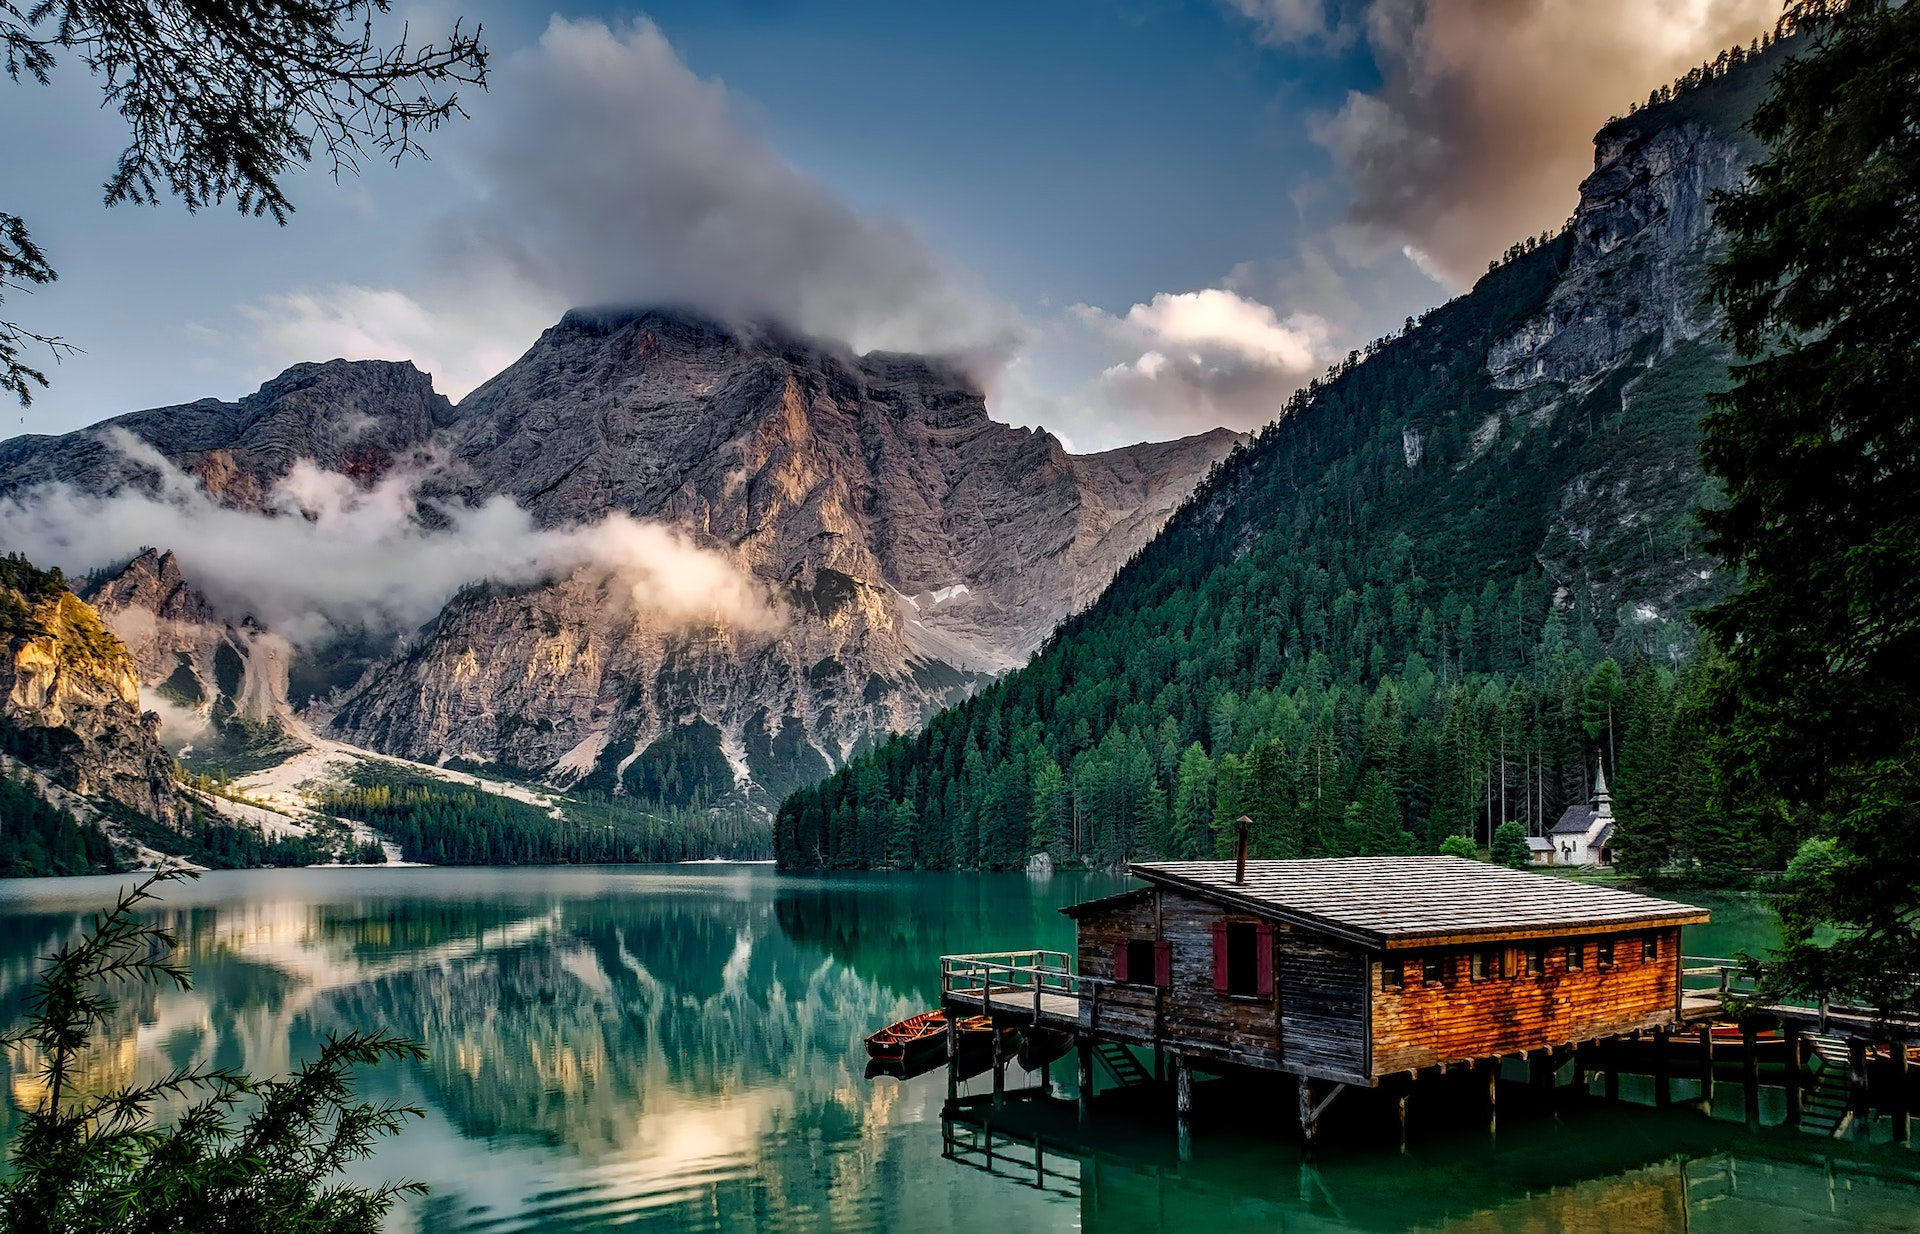
\includegraphics[width=0.7\columnwidth]{assets/images/bilder/pexels-pixabay-147411.jpg}
            \caption{Holzhaus am Gebirgssee}
            \label{fig:holzhaus-am-gebirgssee}
        \end{figure}
    \end{code}
    \tcblower
    \begin{center}
        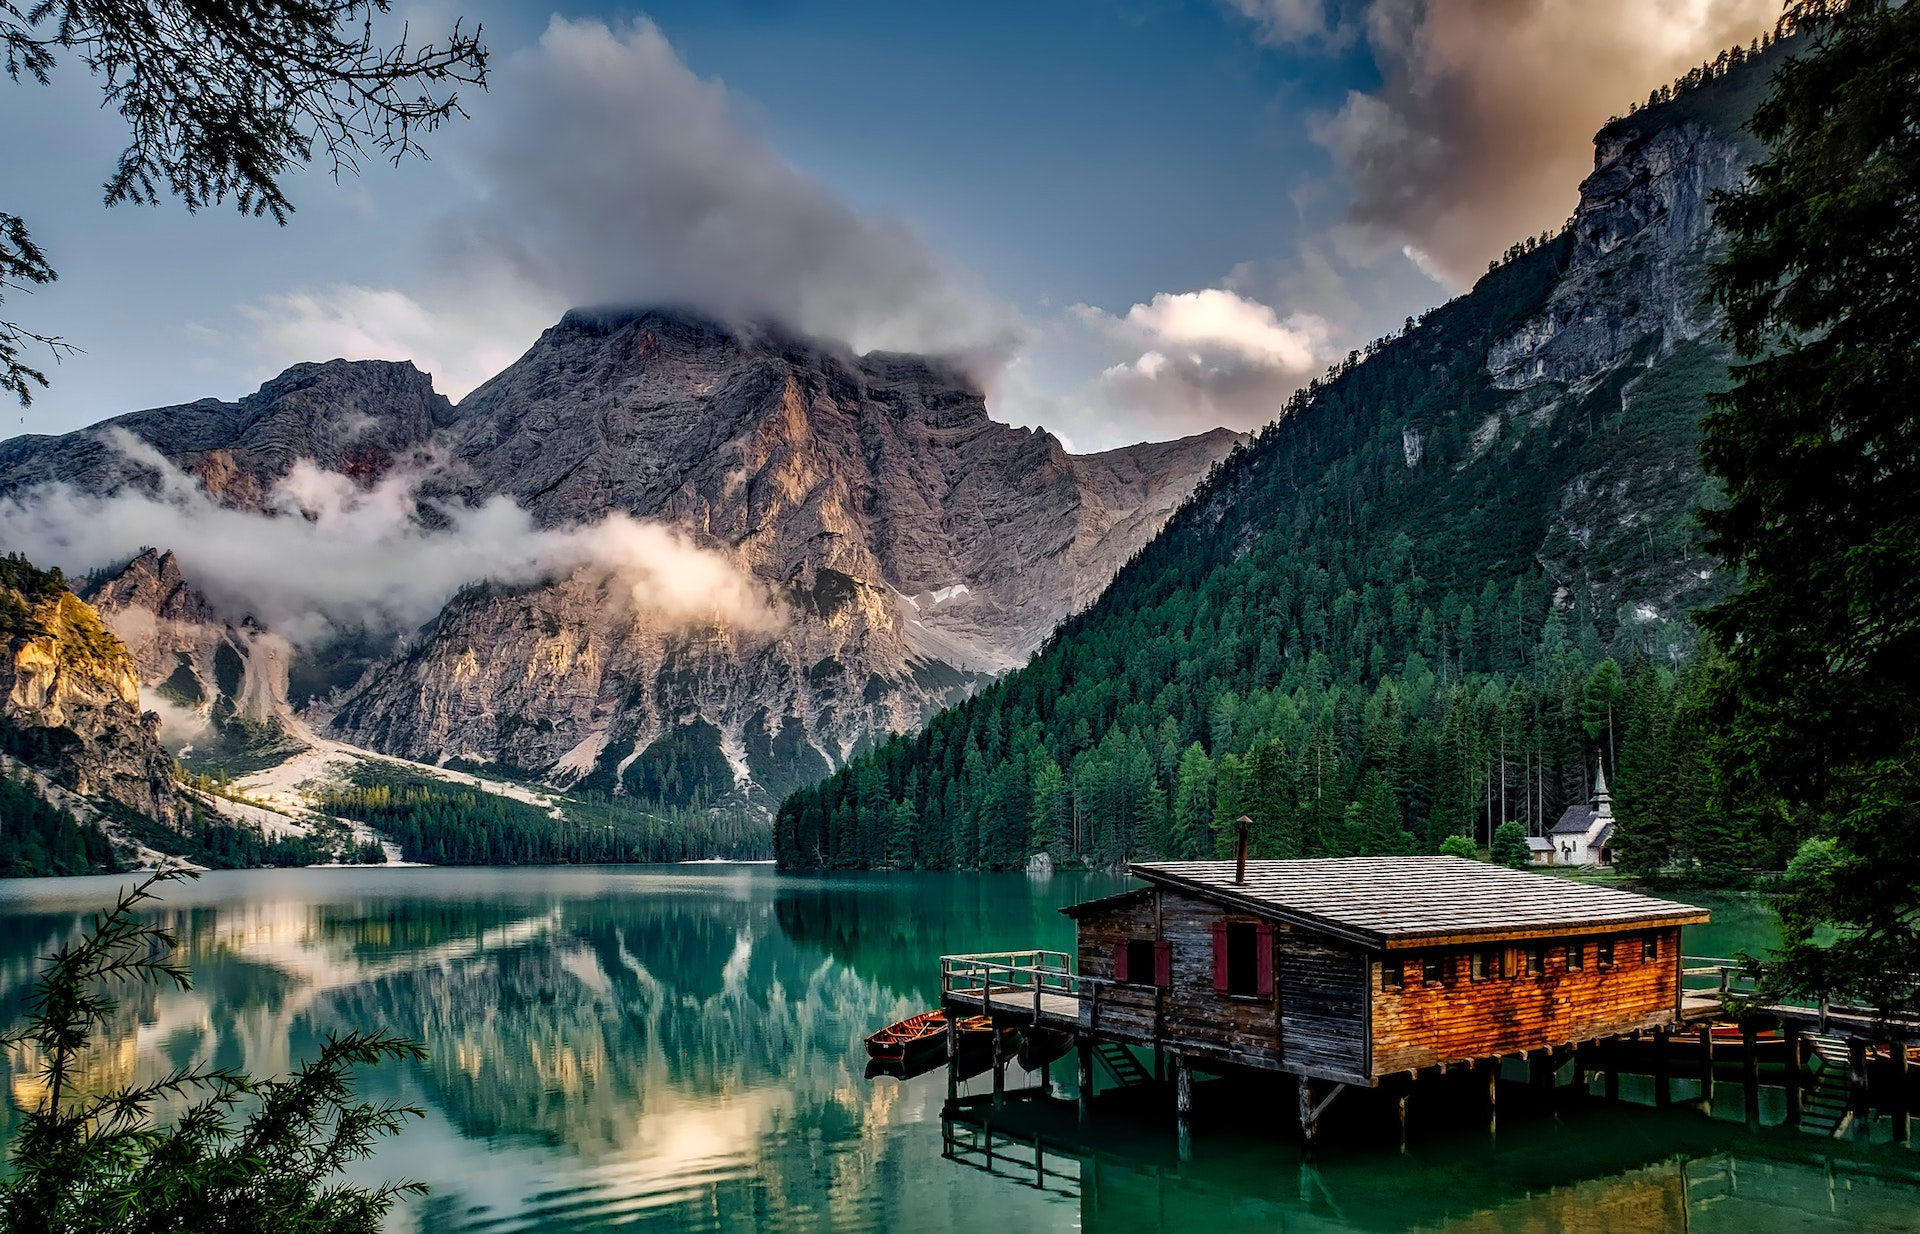
\includegraphics[width=0.7\columnwidth]{assets/images/bilder/pexels-pixabay-147411.jpg}
        \captionof{figure}{Holzhaus am Gebirgssee}
    \end{center}
\end{showcase}

\section{Vektorgrafiken (SVG)}
Sollen komplexe Informationen auf klare und ansprechende Weise wie in Infografiken oder Diagrammen dargestellt werden, eignen sich Vektorgrafiken. Im Gegensatz zu rasterbasierten Formaten (wie JPEG oder PNG) behalten SVG-Grafiken ihre Qualität und Schärfe unabhängig von der Zoomstufe oder Größe. Um SVG-Grafiken in \LaTeX-Dokumente einzufügen, gibt es verschiedene Ansätze, welche im folgenden kurz vorgestellt werden.

\subsection{Konvertierung zu PDF oder EPS}
Werden Grafiken zum Beispiel mit \textit{draw.io}\footnote{\url{https://www.drawio.com/}}, \textit{Inkscape}\footnote{\url{https://inkscape.org/de/}} oder anderen Werkzeugen selbst erstellt, empfiehlt es sich diese auch immer als PDF zu exportieren. Beim Export sollte darauf geachtet werden, dass die Größe des Bildes nur die gezeichneten Inhalte umfasst. Ich persönlich markiere dafür alle gezeichneten Elemente und exportiere nur die Auswahl, wobei es hier verschiedene Möglichkeiten gibt, da beim Markieren Teile des Bildes übersehen werden können. Die als PDF exportierten Bilder können wie normale Bilder mit dem Befehl \mintinline{latex}{\includegraphics[options]{path/to/file.pdf}} in das Dokument eingebettet werden.

\begin{showcase}
    \begin{code}{latex}
        \begin{figure}
            \centering
            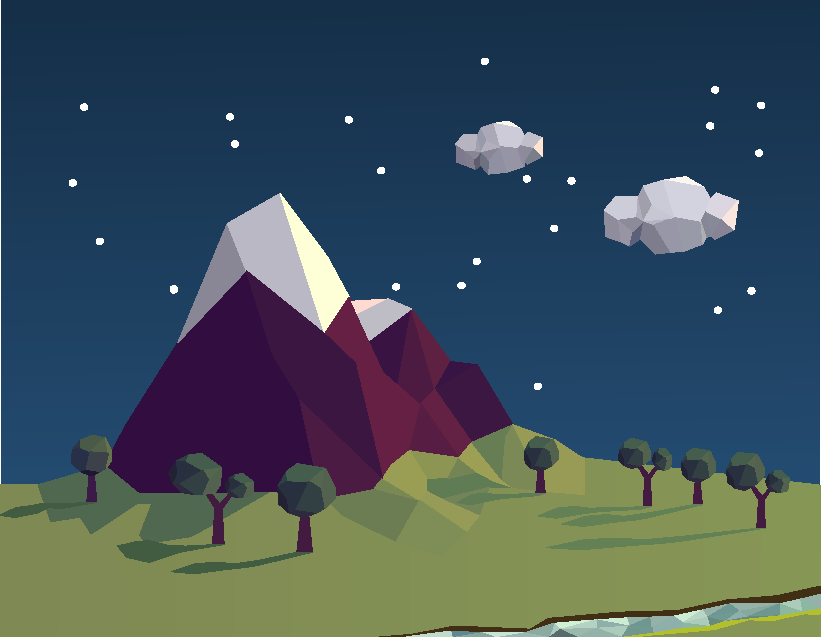
\includegraphics[width=0.5\columnwidth]{assets/images/bilder/landscape.pdf}
            \caption{Landschaft als PDF-Grafik}
            \label{fig:landschaft-als-pdf-grafik}
        \end{figure}        
    \end{code}
    \tcblower
    \begin{center}
        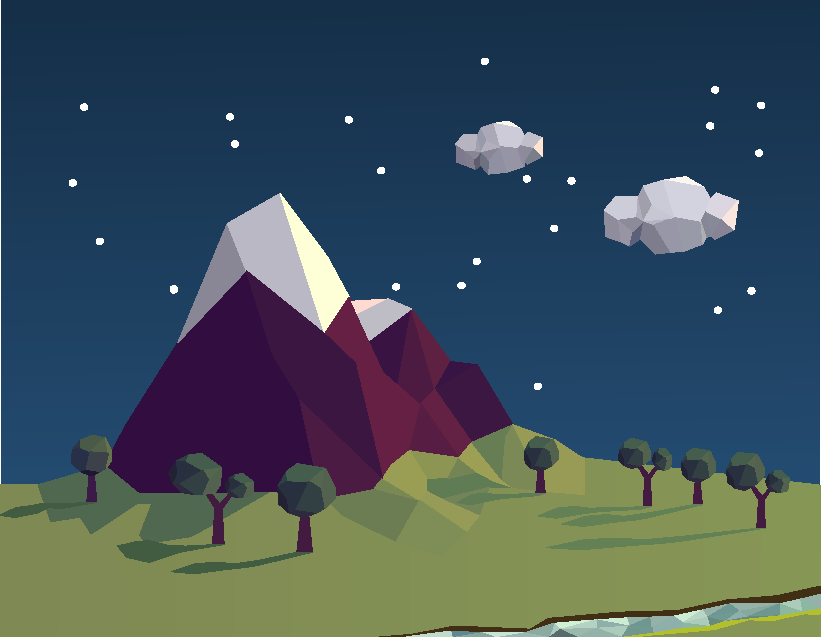
\includegraphics[width=0.5\columnwidth]{assets/images/bilder/landscape.pdf}
        \captionof{figure}{Landschaft als PDF-Grafik}
        \label{fig:landschaft-als-pdf-grafik}
    \end{center}  
\end{showcase}

\subsection{Direkte Verwendung von SVG-Grafiken}
Bei der direkten Verwendung werden die SVG-Grafiken mit den Befehl \mintinline{latex}{\includesvg[options]{path/to/file.svg}} zum Beispiel innerhalb eine Fließumgebung (siehe \autoref{sec:fliessumgebungen}) geladen. \textbf{Durch das Paket wird Inkscape ausgeführt}, weswegen es notwendig ist dieses Programm auf dem Rechner installiert zu haben. Außerdem ist es notwendig für die Ausführung mit z.\,B. \texttt{latexmk} die Option \texttt{-shell-escape} hinzuzufügen. Weitere Informationen für die lokale Einrichtung des Computers zur Verwendung dieses Templates sind auf \url{https://github.com/blackapple113/H-BRS-Thesisvorlage}.\todo{Setup Guide in README}

\begin{showcase}
    \begin{code}{latex}
        \begin{figure}
            \centering
            \includesvg[width=0.5\columnwidth]{assets/images/bilder/landscape.svg}
            \caption{Landschaft als SVG-Grafik}
            \label{fig:landschaft-als-svg-grafik}
        \end{figure}
    \end{code}
    \tcblower
    \begin{center}
        \includesvg[width=0.5\columnwidth]{assets/images/bilder/landscape.svg}
        \captionof{figure}{Landschaft als SVG-Grafik}
        \label{fig:landschaft-als-svg-grafik}
    \end{center}
\end{showcase}

\subsection{Vergleich SVG- vs. PDF-Grafik}
\label{subsec:vergleich-svg-vs-pdf-grafik}
Werden SVG-Grafiken direkt in \LaTeX verwendet werden sie in ein \LaTeX verständliches Format umgewandelt. Dabei können ungewollte Formatierungsprobleme innerhalb der Grafik auftreten. Als Beispiel werden im Folgenden zwei Diagramme gezeigt. Das Diagramm auf der linken Seite wurde als PDF importiert und das Diagramm auf der rechten Seite als SVG-Grafik. Es sei gesagt, dass die klasse \texttt{hbrs-thesis} schon einige Optionen für die bessere Verwendung von SVG-Grafiken eingestellt hat. Dennoch kann es, wie im Beispiel gezeigt, zu Problemen kommen.

\begin{figure}[H]
    \begin{minipage}[c]{0.48\columnwidth}
        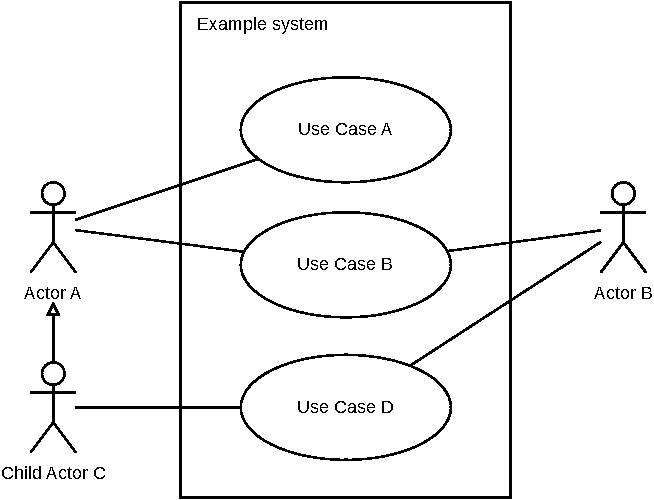
\includegraphics[width=\linewidth]{assets/images/bilder/UML-exmaple.pdf}
        \subcaption{PDF-Grafik}
        \label{subfig:pdf-grafik}
    \end{minipage}
    \hfill
    \begin{minipage}[c]{0.48\columnwidth}
        \includesvg[width=\linewidth]{assets/images/bilder/UML-example.svg}
        \subcaption{SVG-Grafik}
        \label{subfig:svg-grafik}
    \end{minipage}       
    \caption{SVG- vs. PDF-Grafik} 
\end{figure}

Die in diesem Beispiel gezeigten Unterschiede sind so gering, dass sie bei der ersten Kontrolle vielleicht gar nicht auffallen. Bei genauerer Betrachtung kann man erkennen, dass die Beschriftungen der einzelnen Aktoren in der SVG-Grafik nicht ausgeschrieben sind. Es fehlen also relevante Informationen, die in der PDF-Grafik enthalten sind. Trotzdem handelt es sich bei der PDF-Datei um eine Vektorgrafik, welche also keinen Qualitätsverlust aufweist.

\section{Teilbilder}
Wie in \autoref{subsec:vergleich-svg-vs-pdf-grafik} als Vergleichsabbildung zwischen SVG- und PDF-Grafiken verwendet, müssen manchmal mehrere Bilder nebeneinander platziert werden. Diese können unabhängig voneinander Beschriftet werden oder als Teil der übergeordneten Fließumgebung. Um Bilder nebeneinander platzieren zu können, wird die Umgebung \texttt{minipage} (siehe \autoref{sec:minipage}) verwendet. Im Folgenden ein paar Beispiele für die Anordnung von Bildern in einer Reihe.

\begin{showcase}
    \begin{code}{latex}
        \begin{figure}
            \centering
            \begin{minipage}[c]{0.49\columnwidth}
                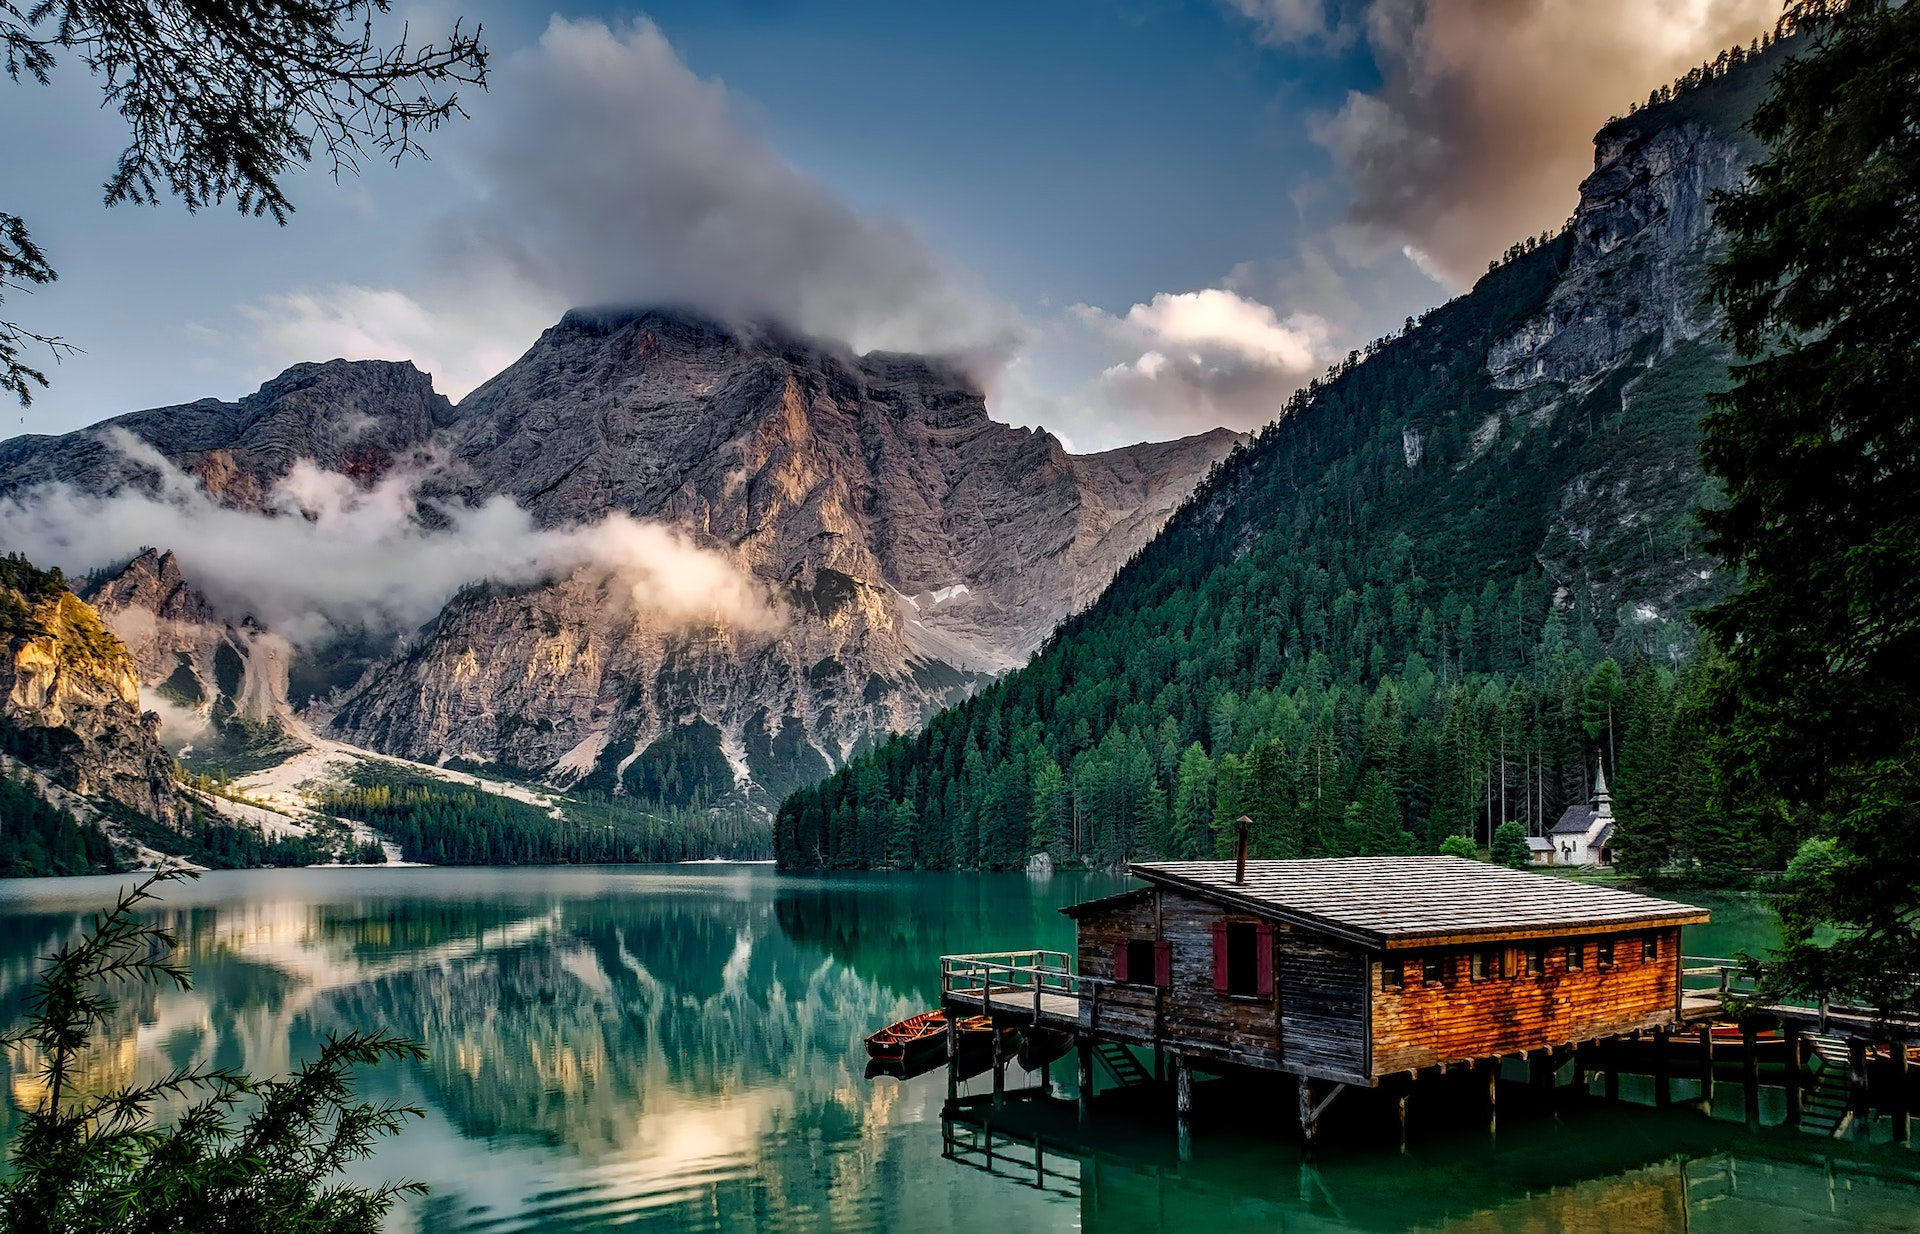
\includegraphics[width=\linewidth]{assets/images/bilder/pexels-pixabay-147411.jpg}
                \subcaption{Holzhütte am Gebirgssee}
            \end{minipage}
            \hfill
            \begin{minipage}[c]{0.49\columnwidth}
                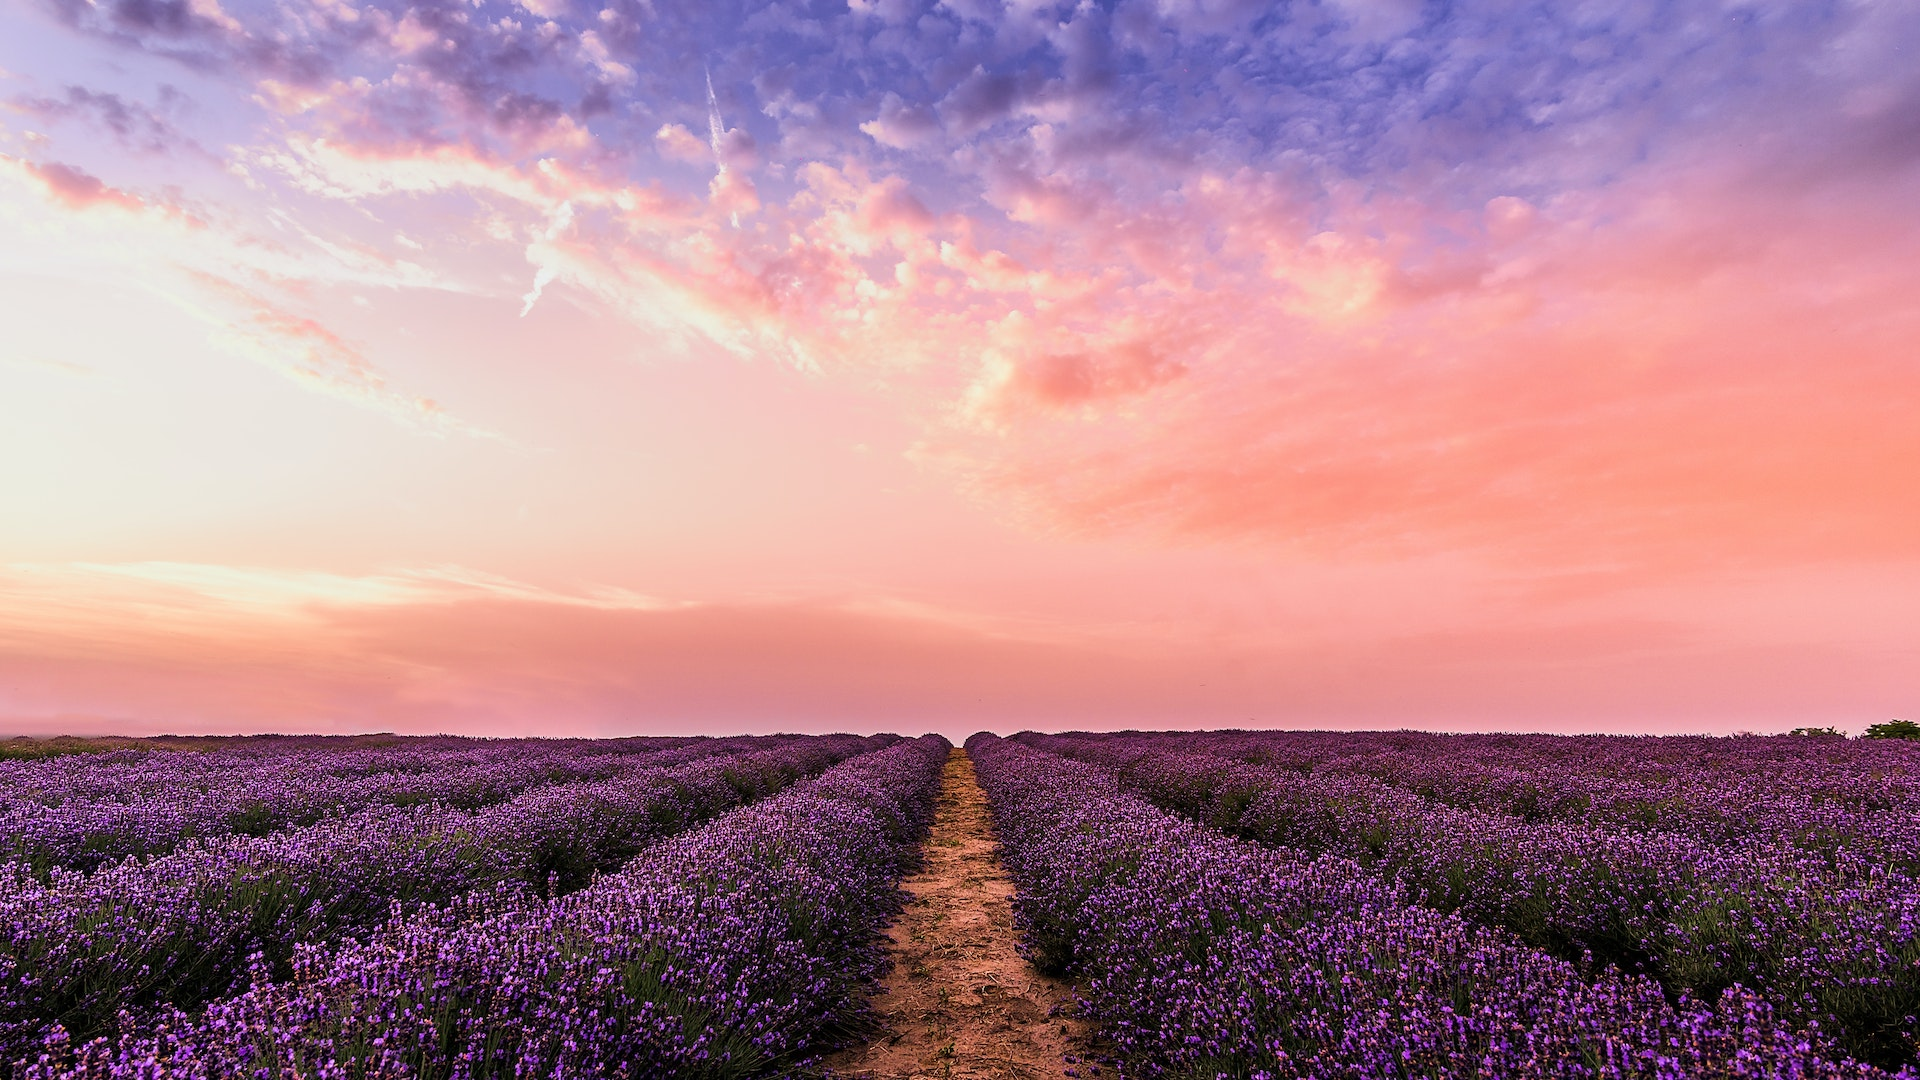
\includegraphics[width=\linewidth]{assets/images/bilder/pexels-david-bartus-1166209.jpg}
                \subcaption{Lavendelfelder im Sonnenuntergang}
            \end{minipage}
            \caption{Zwei farbenprächtige Naturfotografien}
        \end{figure}
    \end{code}
    \tcblower
    \begin{center}
        \captionsetup{type=figure}
        \begin{subfigure}{0.49\columnwidth}
            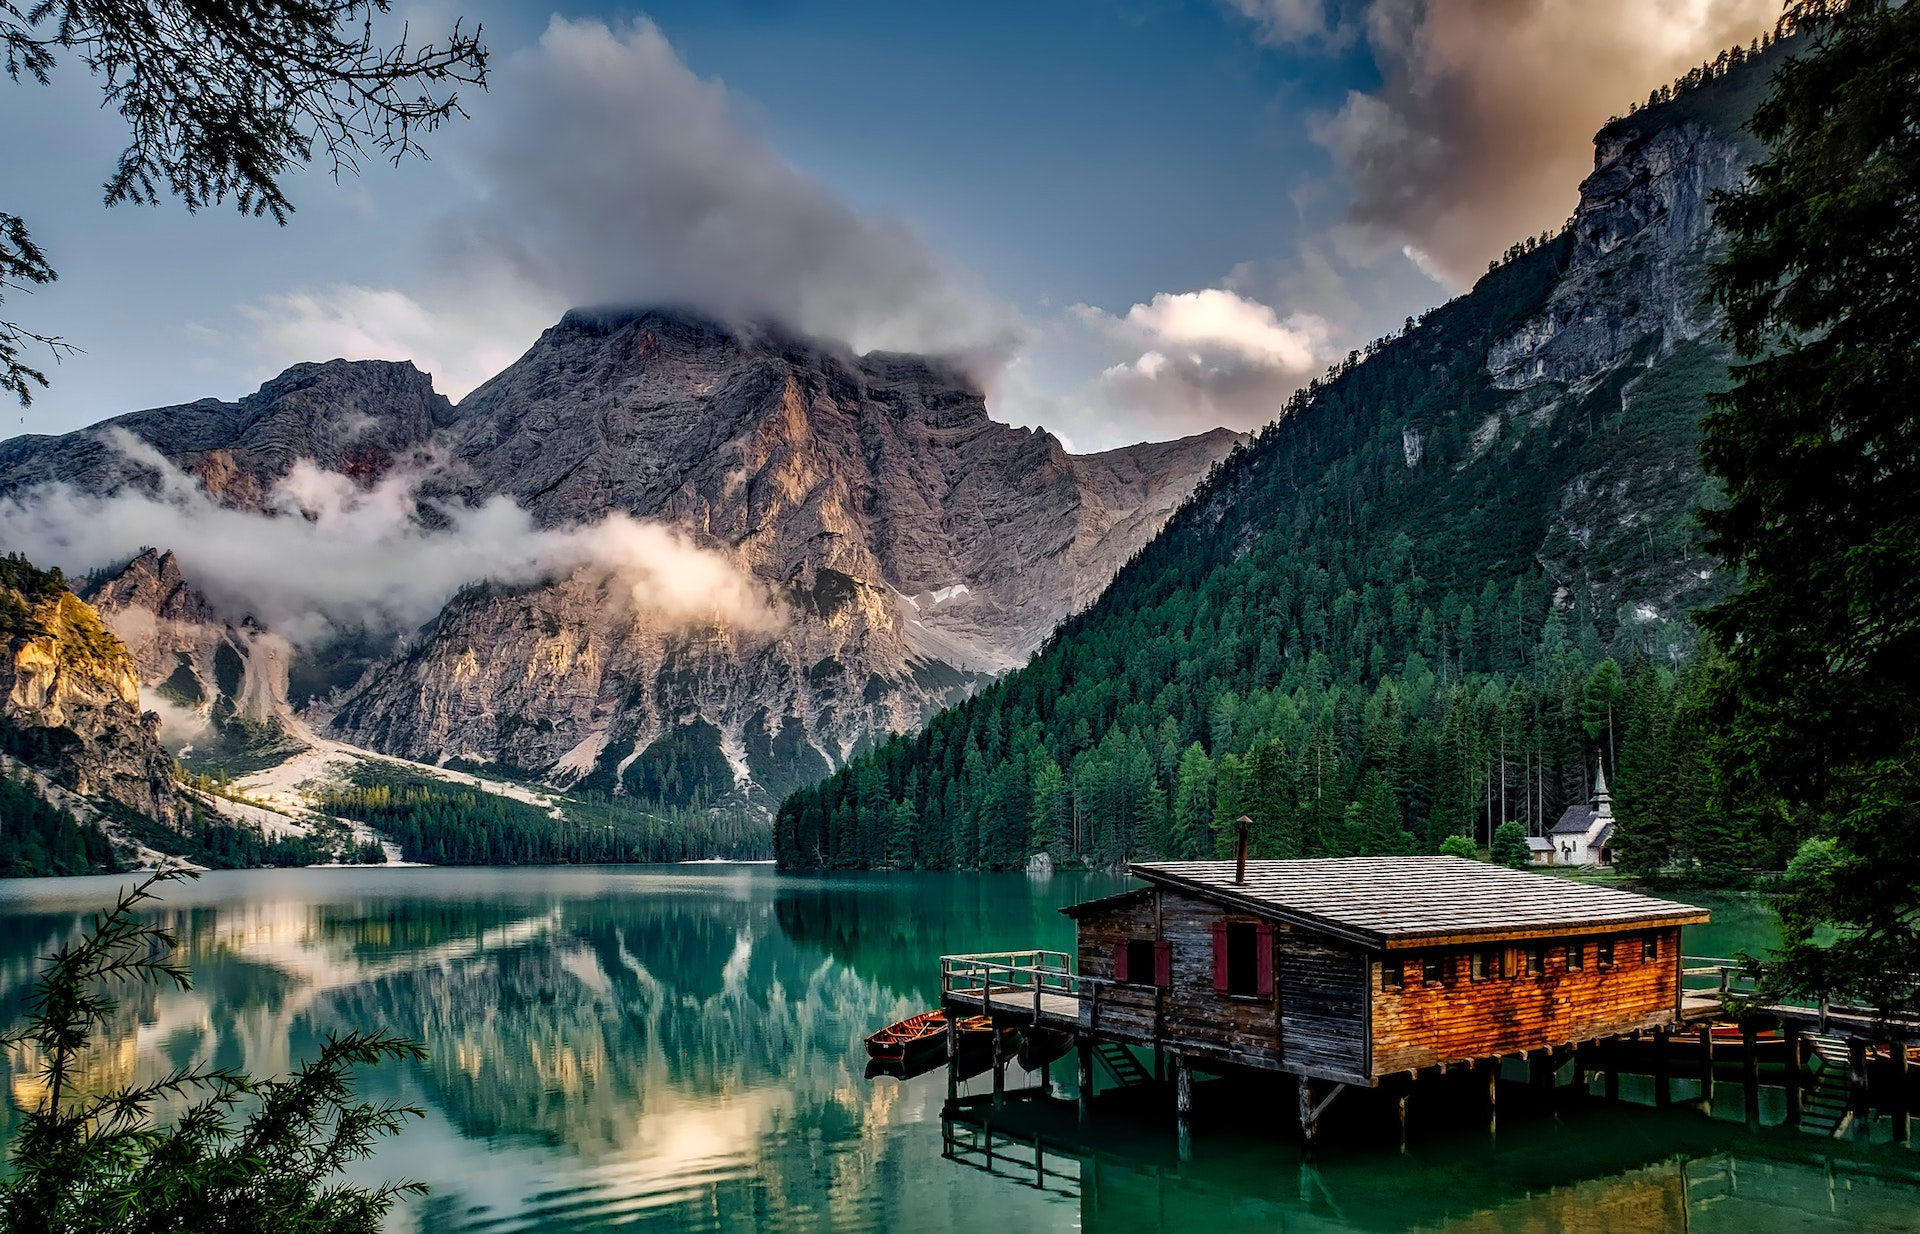
\includegraphics[width=\linewidth]{assets/images/bilder/pexels-pixabay-147411.jpg}
            \caption{Holzhütte am Gebirgssee}
        \end{subfigure}
        \hfill
        \begin{subfigure}{0.49\columnwidth}
            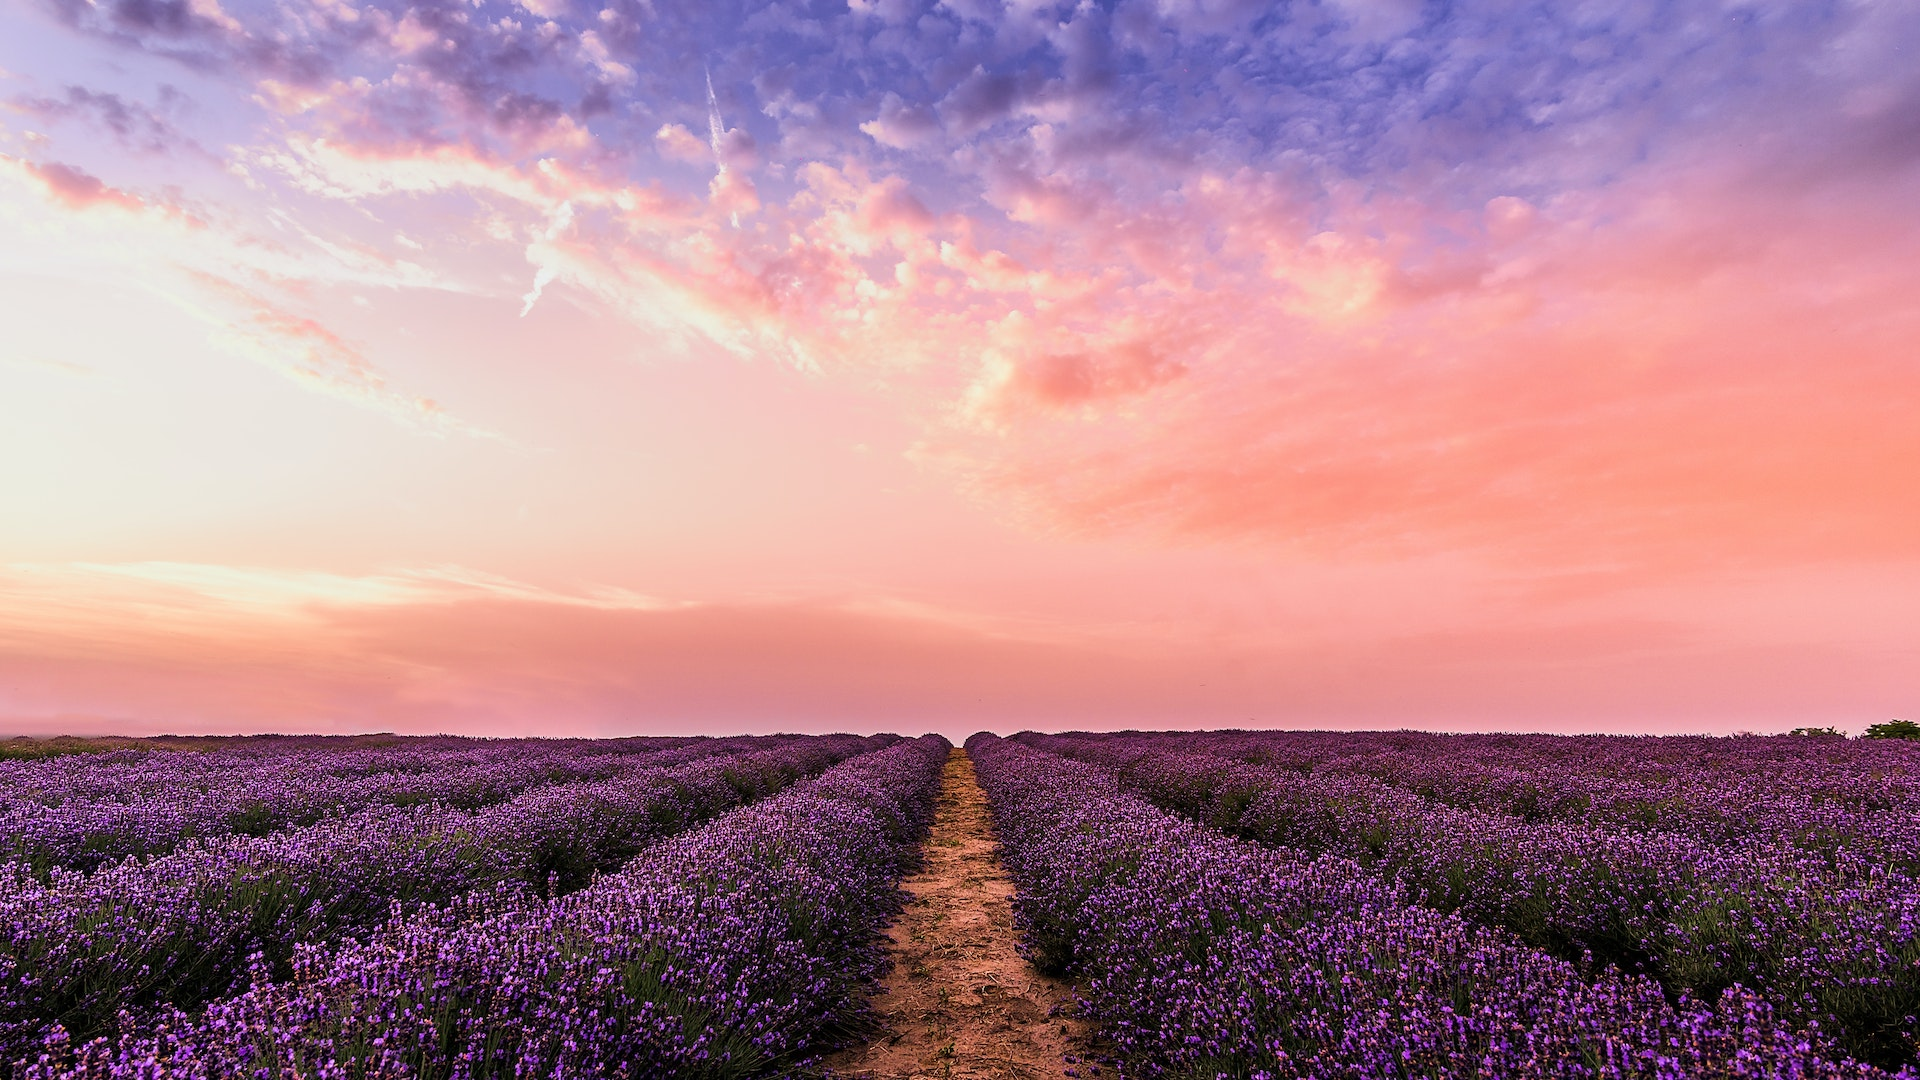
\includegraphics[width=\linewidth]{assets/images/bilder/pexels-david-bartus-1166209.jpg}
            \caption{Lavendelfelder im Sonnenuntergang}
        \end{subfigure}
        \captionof{figure}{Zwei farbenprächtige Landschaftsfotos}
    \end{center}
\end{showcase}

\begin{showcase}
    \begin{code}{latex}
        \begin{figure}[H]
            \begin{minipage}[c]{0.27\columnwidth}
                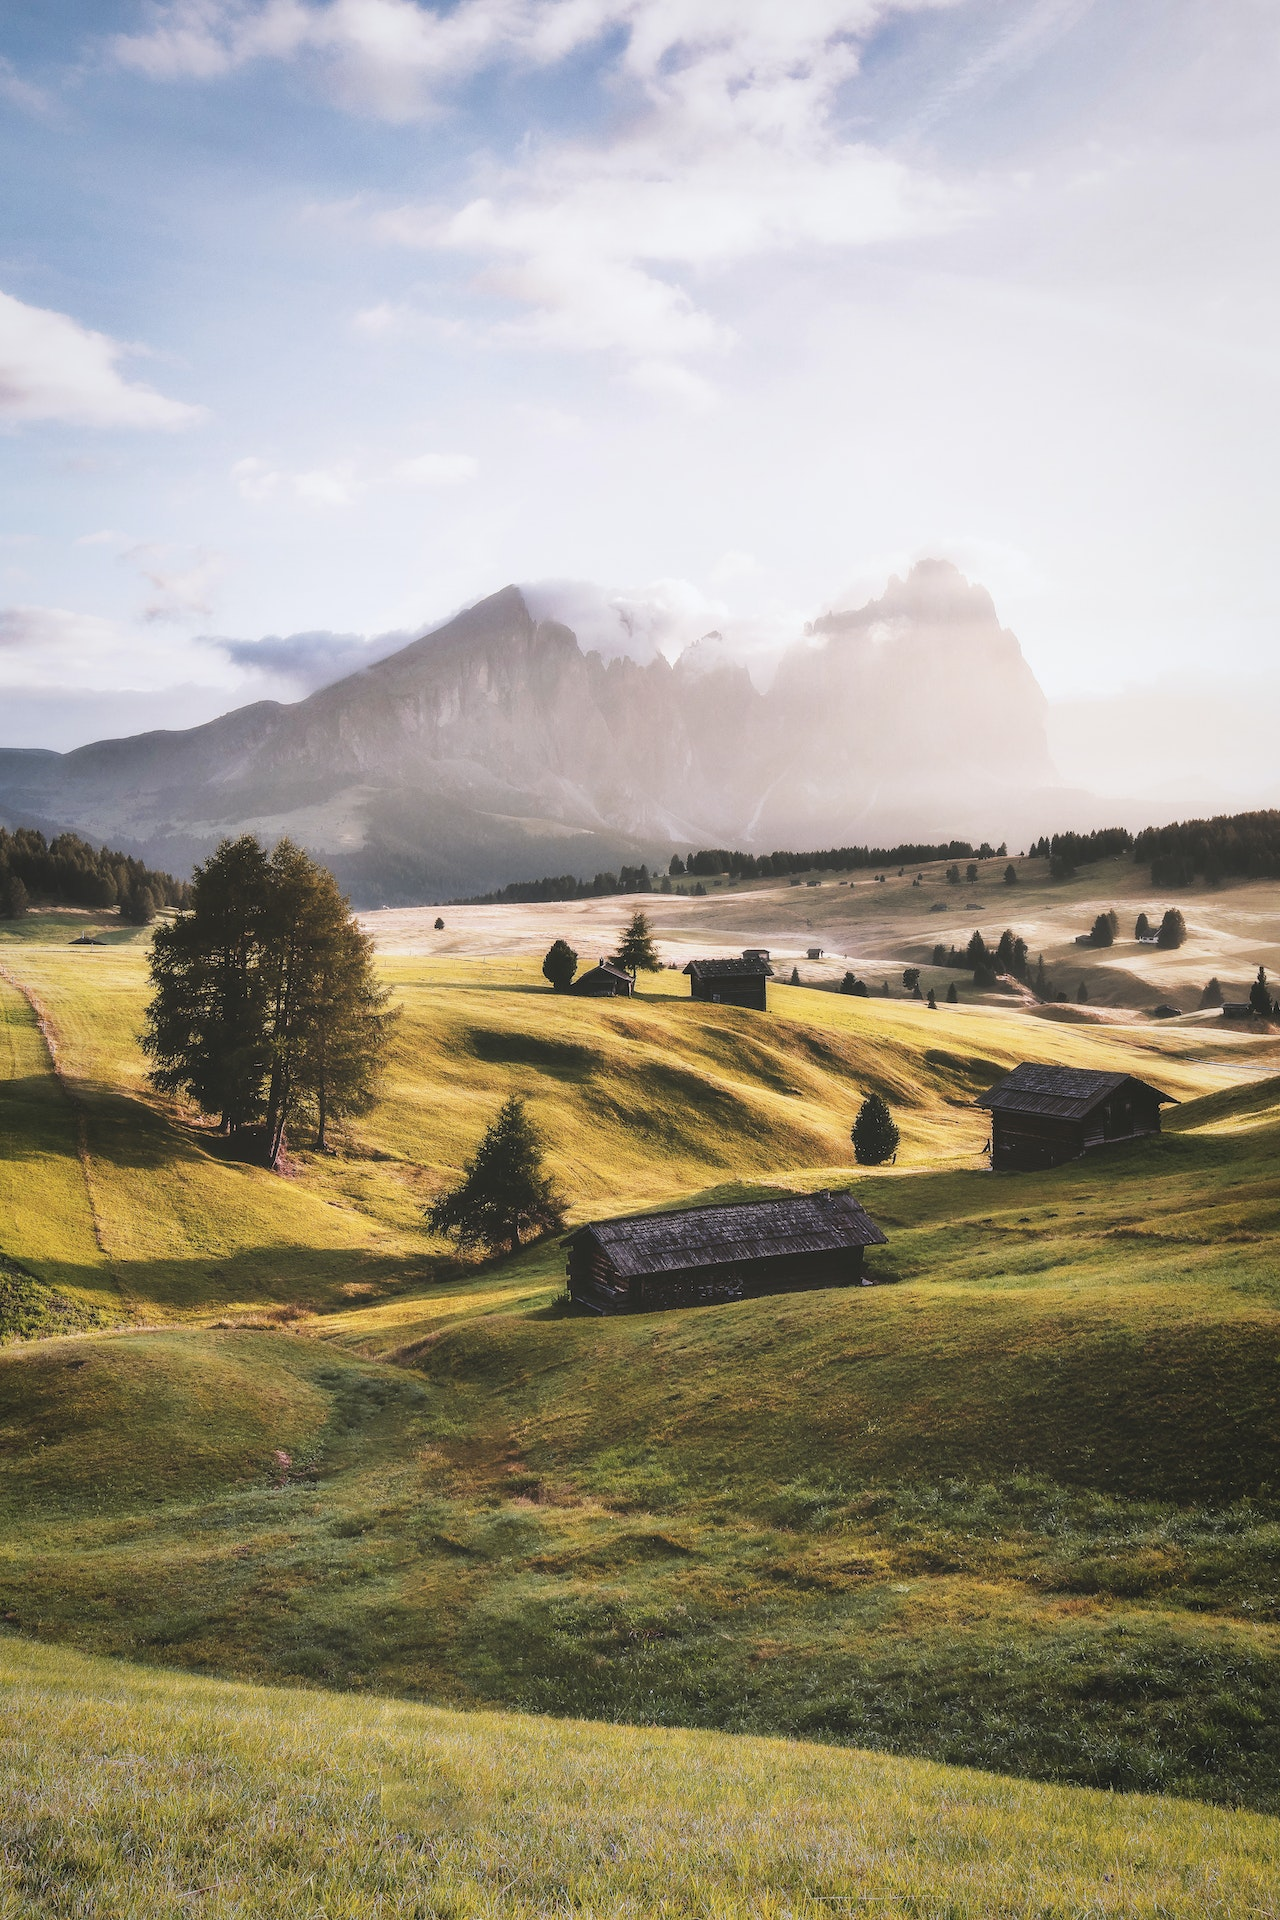
\includegraphics[width=\linewidth,height=6cm,keepaspectratio]{assets/images/bilder/pexels-eberhard-grossgasteiger-2437291.jpg}
                \subcaption{Hügelige Landschaft}
            \end{minipage}
            \hfill
            \begin{minipage}[c]{0.72\columnwidth}
                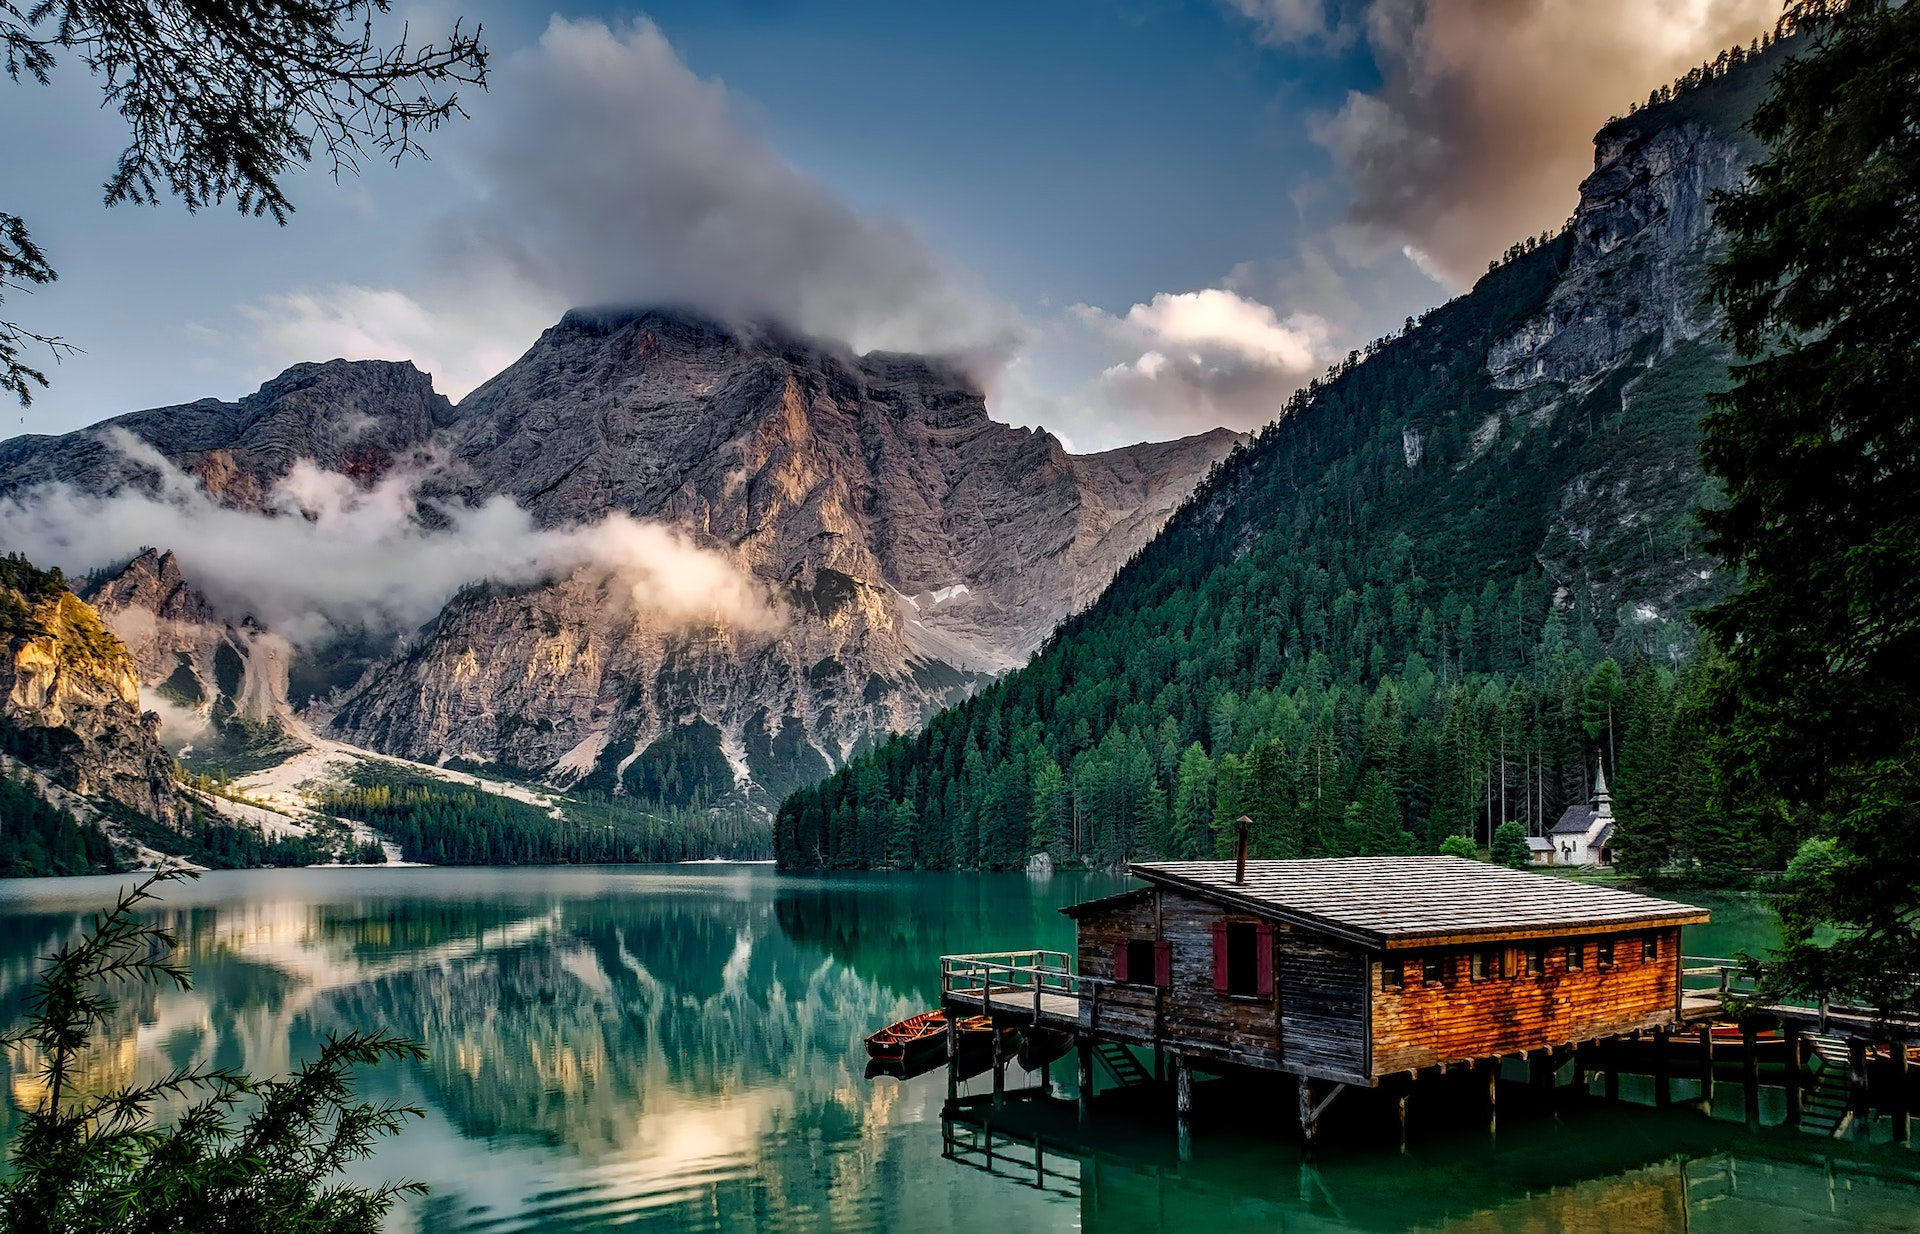
\includegraphics[width=\linewidth,height=6cm,keepaspectratio]{assets/images/bilder/pexels-pixabay-147411.jpg}
                \subcaption{Holzhütte am Gebirgssee}
            \end{minipage}
            \caption{Zwei farbenprächtige Landschaftsfotos}
        \end{figure}
    \end{code}
    \tcblower
    \begin{center}
        \captionsetup{type=figure}
        \begin{subfigure}{0.27\columnwidth}
            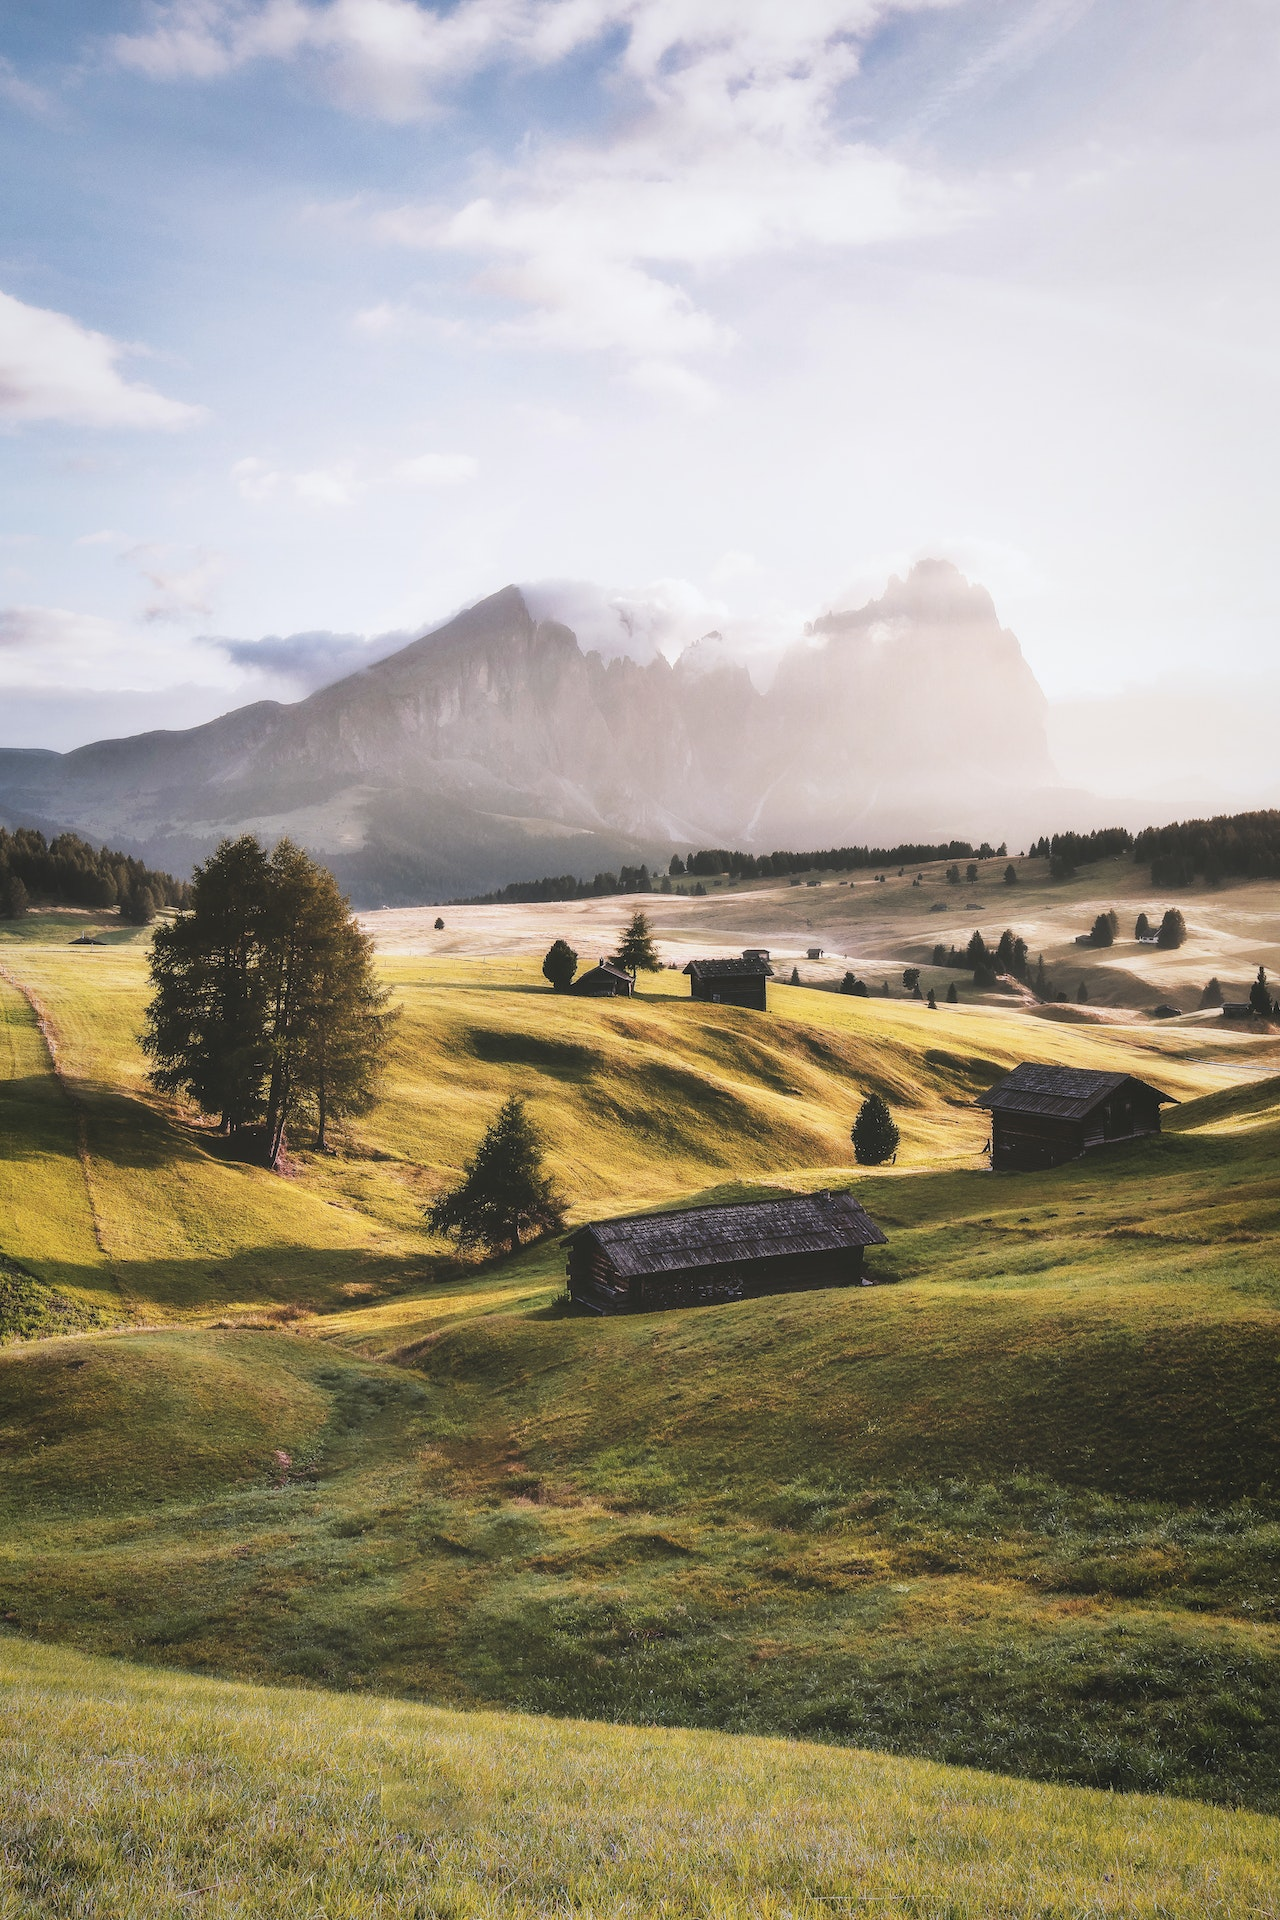
\includegraphics[width=\linewidth,height=6cm,keepaspectratio]{assets/images/bilder/pexels-eberhard-grossgasteiger-2437291.jpg}
            \caption{Hügelige Landschaft}
        \end{subfigure}
        \hfill
        \begin{subfigure}{0.72\columnwidth}
            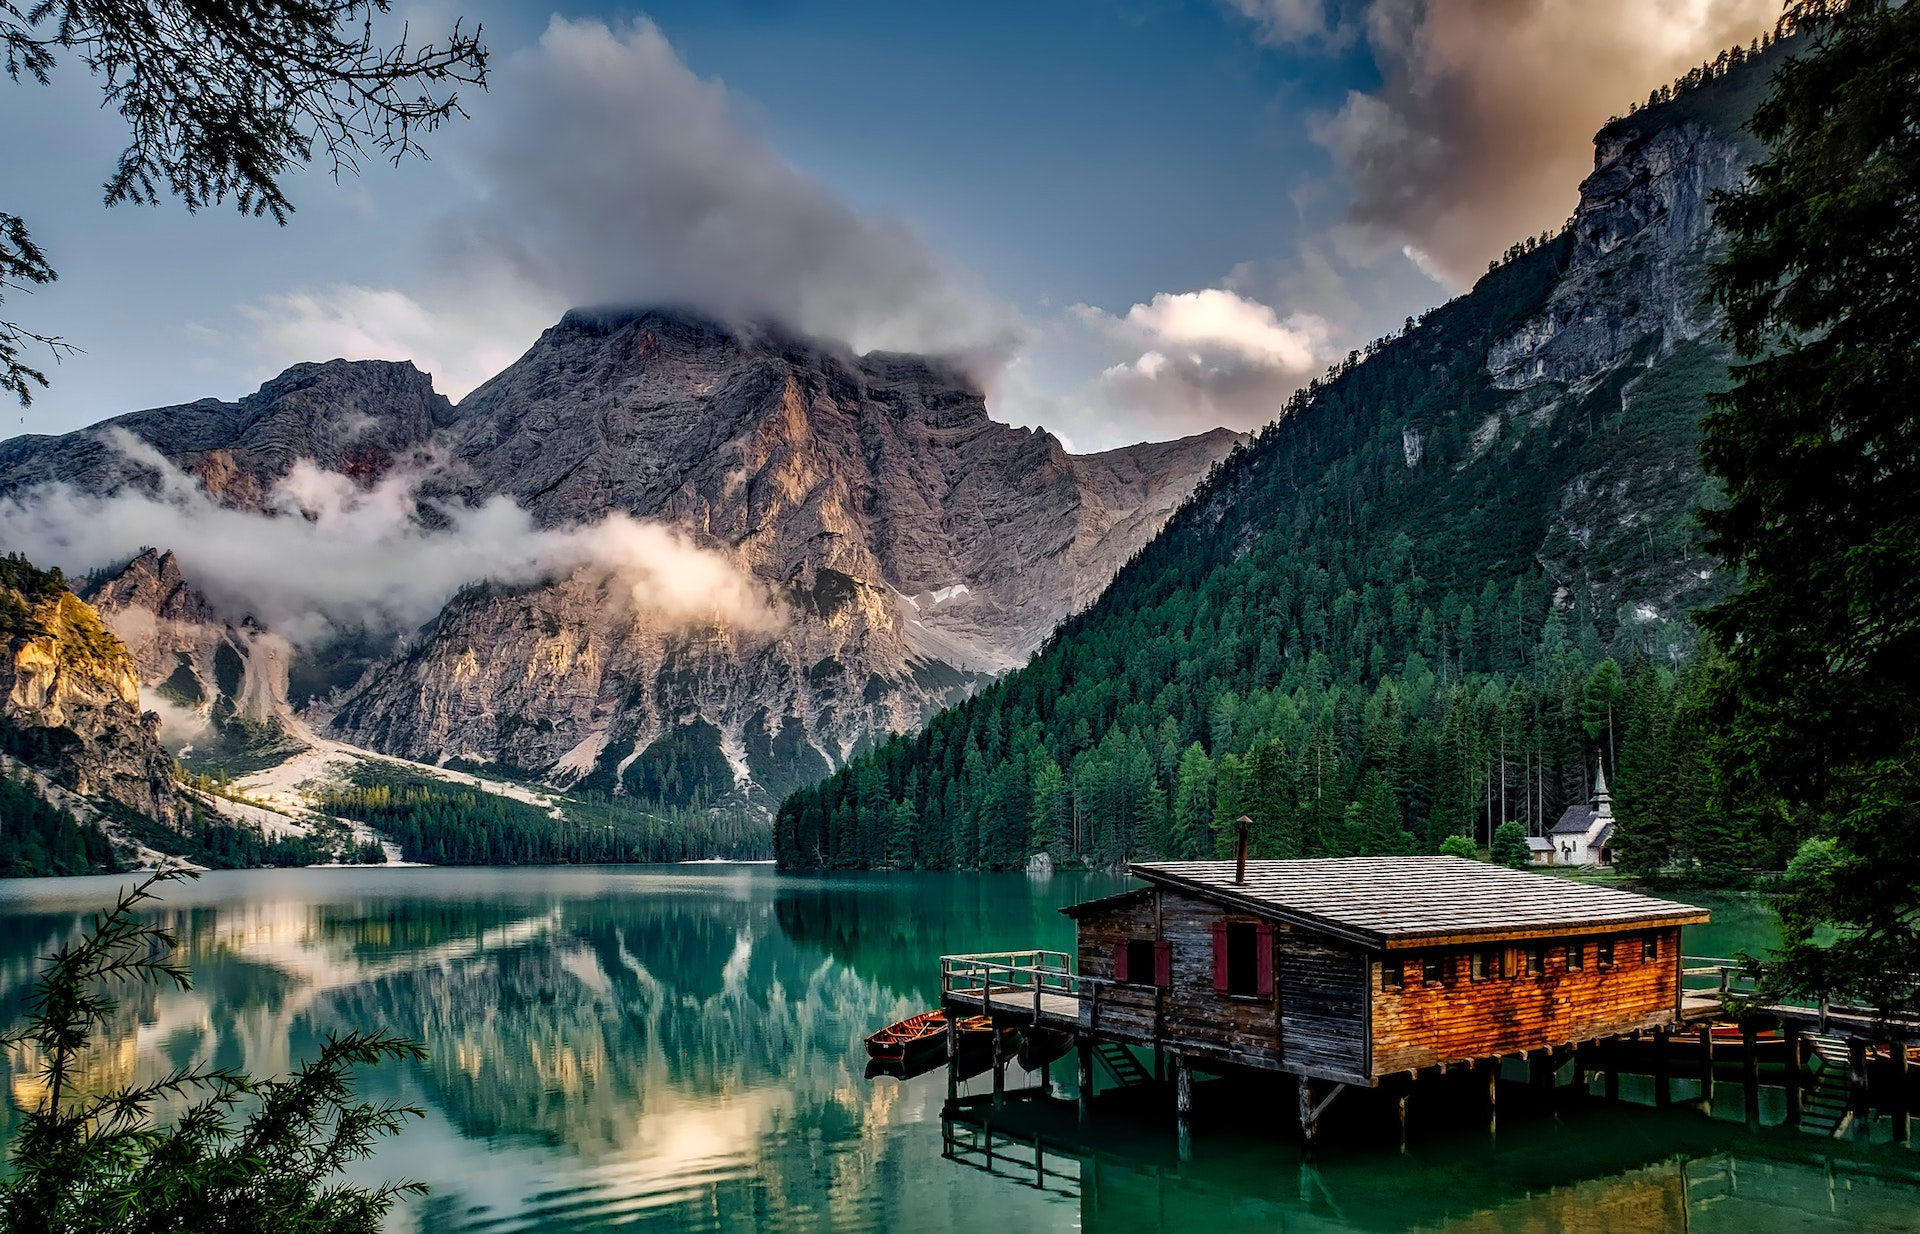
\includegraphics[width=\linewidth,height=6cm,keepaspectratio]{assets/images/bilder/pexels-pixabay-147411.jpg}
            \caption{Holzhütte am Gebirgssee}
        \end{subfigure}
        \captionof{figure}{Zwei farbenprächtige Landschaftsfotos}
    \end{center}
\end{showcase}

\section{Wrapfigure}
Die \texttt{wrapfigure}-Umgebung in \LaTeX ermöglicht es, Bilder in den Textfluss einzufügen und den umgebenden Text harmonisch um die Abbildung zu positionieren. Im Gegensatz zu herkömmlichen Fließumgebungen, die eine separate Zeile für Abbildungen reservieren, kann \texttt{wrapfigure} das Bild links oder rechts vom Text umfließen lassen. Dies ist besonders nützlich, wenn ein Bild eng mit dem umgebenden Text verbunden ist und eine nahtlose Integration gewünscht ist. Wie in einer normalen Fließumgebung können Beschriftungen mit \mintinline{latex}{\caption{}} gesetzt werden. Die Verwendung von \texttt{wrapfigure}-Umgebung erfordert eine sorgfältige Handhabung, da sie den Textfluss beeinflussen kann. Sie sollte mit Bedacht verwendet werden, um sicherzustellen, dass der Lesefluss und das Layout des Dokuments nicht gestört werden. Für weitere Informationen siehe \url{https://ctan.org/pkg/wrapfig2}.

\begin{table}[H]
    \centering
    \captionabove{Optionen für \texttt{wrapfigure} und \texttt{wraptable}}
    \begin{tblr}{lll}
        \toprule
        \SetCell[c=2]{c}\textbf{Option} & & \textbf{Platzierung} \\
        \midrule
        r & R & rechts, fließend rechts \\
        l & L & links, fließend links \\
        i & I & Innenseite, fließend Innenseite  \\
        o & O & Außenseite, fließend Außenseite \\
        \bottomrule
    \end{tblr}
\end{table}

\begin{showcase}
    …
    \begin{code}{latex}
        \begin{wrapfigure}{r}{0.5\columnwidth}
            \centering
            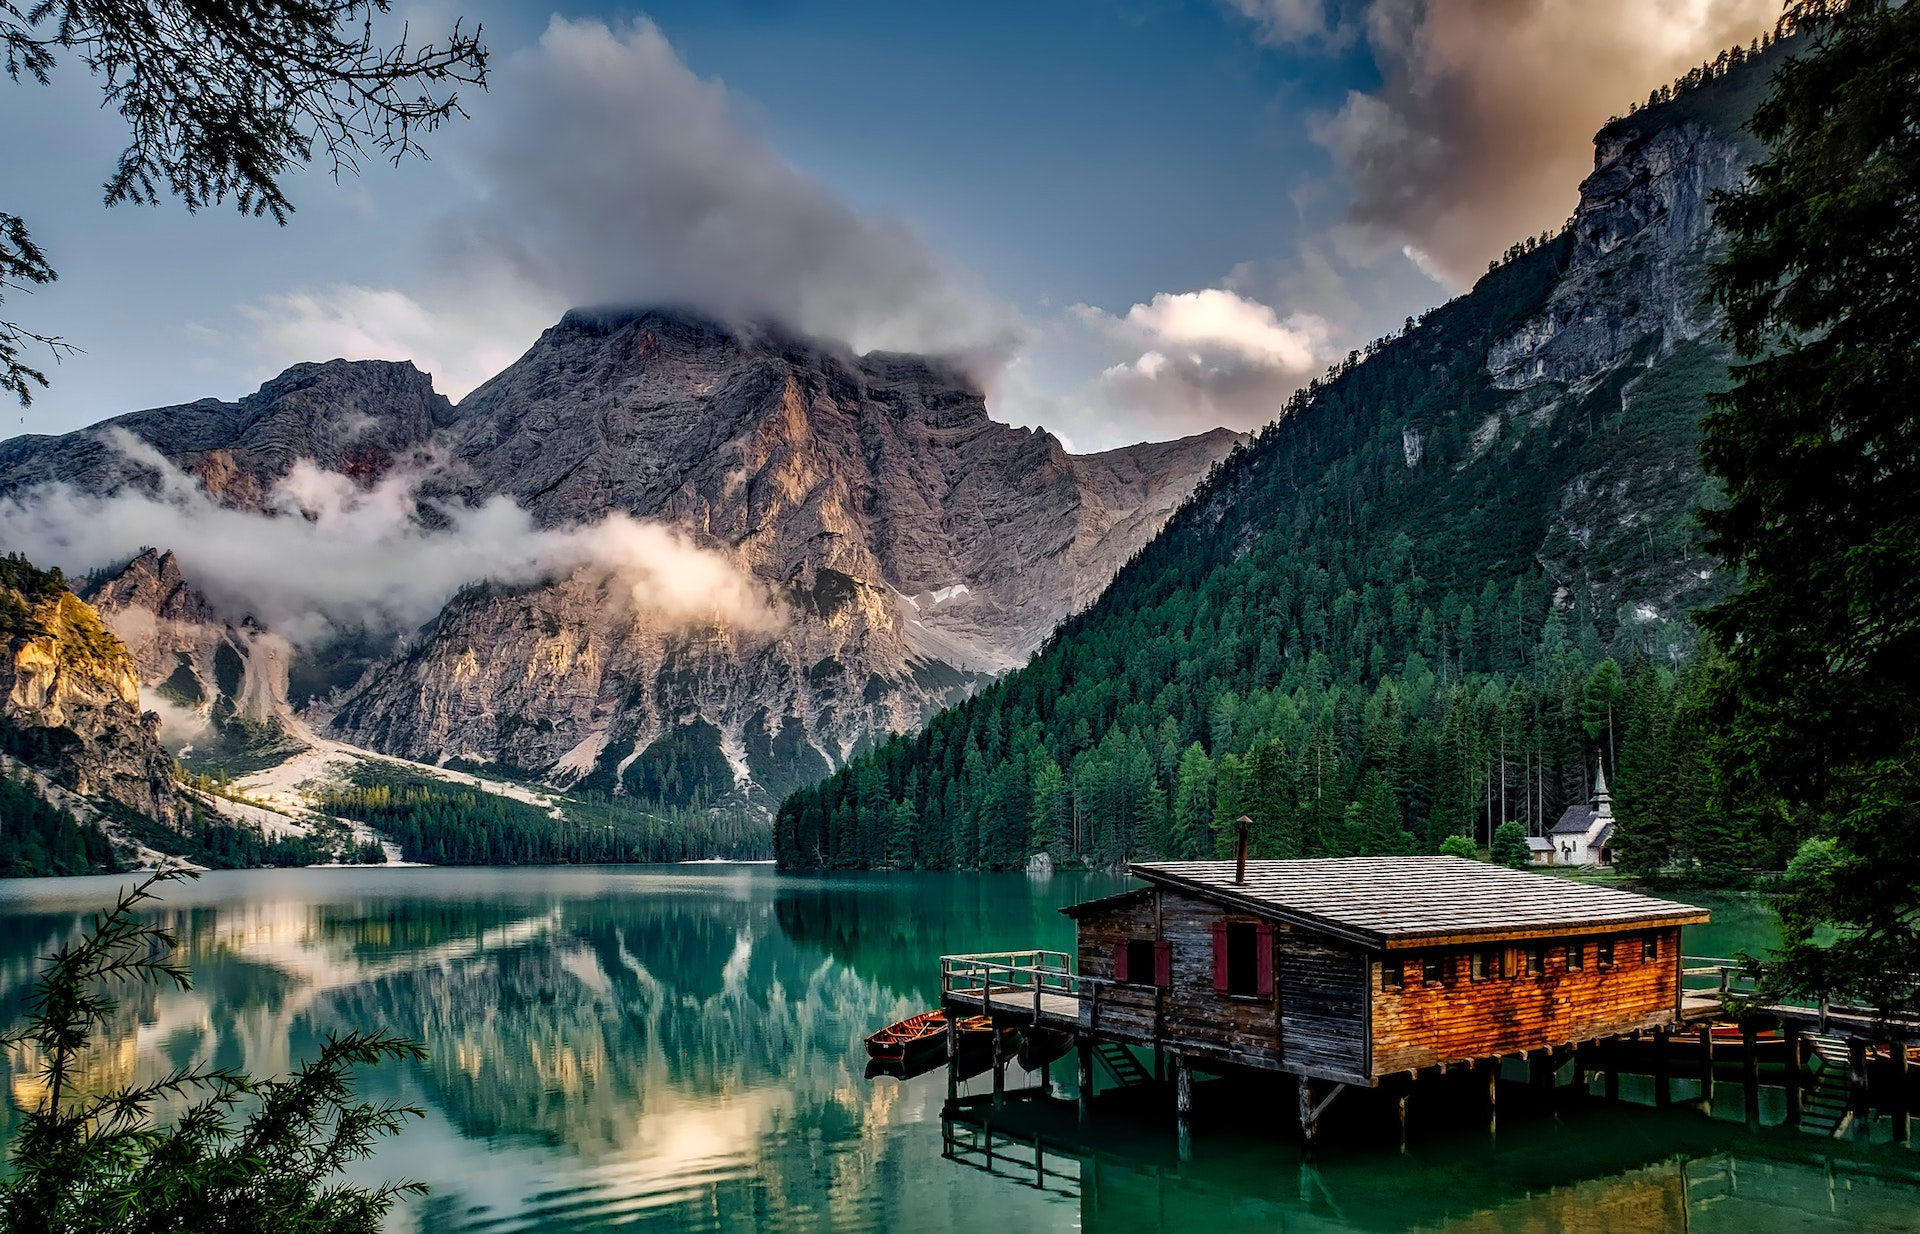
\includegraphics[width=0.5\columnwidth]{assets/images/bilder/pexels-pixabay-147411.jpg}
        \end{wrapfigure}
    \end{code}
    …
    \tcblower
    \begin{wrapfigure}{r}{0.5\columnwidth}
        \centering
        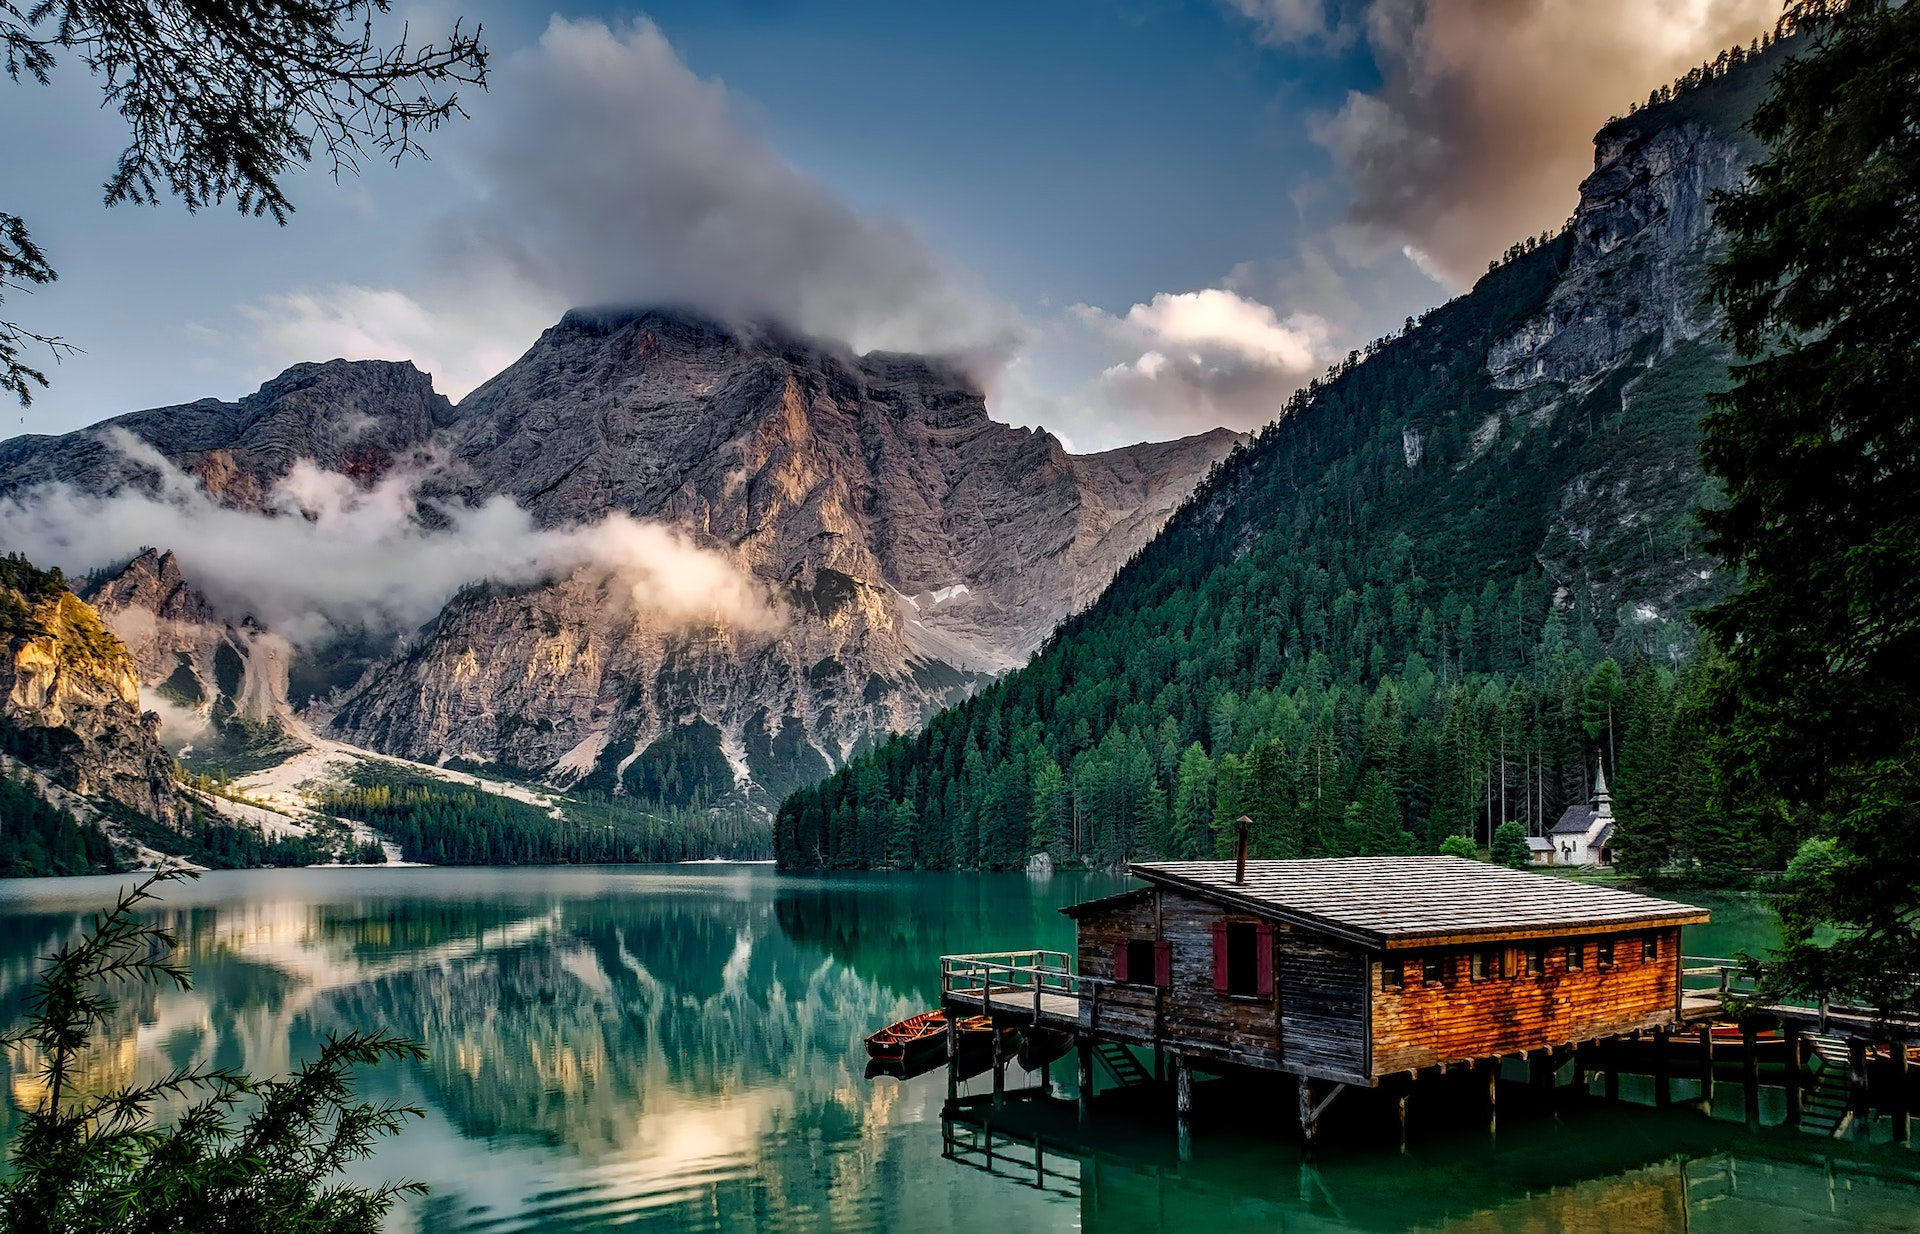
\includegraphics[width=0.5\columnwidth]{assets/images/bilder/pexels-pixabay-147411.jpg}
        \caption{Hütte am See vor dem Kursivgebirge}
    \end{wrapfigure}
    Weit hinten, hinter den Wortbergen, fern der Länder Vokalien und Konsonantien leben die Blindtexte. Abgeschieden wohnen sie in Buchstabhausen an der Küste des Semantik, eines großen Sprachozeans. Nicht einmal von der allmächtigen Interpunktion werden die Blindtexte beherrscht – ein geradezu unorthographisches Leben. Eines Tages aber beschloß eine kleine Zeile Blindtext, ihr Name war Lorem Ipsum, hinaus zu gehen in die weite Grammatik. Der große Oxmox riet ihr davon ab, da es dort wimmele von bösen Kommata, wilden Fragezeichen und hinterhältigen Semikoli, doch das Blindtextchen ließ sich nicht beirren. Es packte seine sieben Versalien, schob sich sein Initial in den Gürtel und machte sich auf den Weg. Als es die ersten Hügel des Kursivgebirges erklommen hatte, warf es einen letzten Blick zurück auf die Skyline seiner Heimatstadt Buchstabhausen, die Headline von Alphabetdorf und die Subline seiner eigenen Straße, der Zeilengasse. Wehmütig lief ihm eine rhetorische Frage über die Wange, dann setzte es seinen Weg fort.
\end{showcase}
\chapter{Code}
Diese Klasse verwendet das Paket \texttt{minted} (siehe \url{https://www.ctan.org/pkg/minted}) für Syntax Highlighting. Das Paket basiert auf \textit{Pygments} (siehe \url{https://pygments.org/}) welches mit Python auf dem System installiert sein sollte, solange kein Docker-Container zum Bauen bereitsteht. Außerdem muss für das Kompilieren die Option \texttt{-shell-escape} hinzugefügt werden, also \mintinline{bash}{latexmk -shell-escape file.tex}. Die von \texttt{minted} unterstützten sprachen für Highlighting sind unter folgender Adresse aufgelistet: \url{https://pygments.org/docs/lexers/}

\section{Inline Code}
Code, der im Text stehen soll, kann auf verschiedene Arten erreicht werden. Die einfachste ist die Verwendung von \texttt{\textbackslash{}texttt\{…\}}. Dabei wird allerdings kein Syntax Highlighting verwendet. Der Text wird innerhalb dieser Umgebung nur an Leerzeichen umgebrochen und nicht innerhalb der Wörter.

Eine weitere Möglichkeit für Syntax Highlighting im Fließtext bietet \texttt{minted} mit dem Befehl \mintinline{latex}{\mintinline{sprache}{code}}. Dieser Befehl kann zusätzlich an vorgegebenen Stellen den Text umbrechen, was dennoch zu Problemen bei der Formatierung am Rand führen kann.

\begin{information}
    Overleaf unterstützt die \mintinline{latex}{\mintinline{sprache}{code}} nicht. Aus diesem Grund sollte in Overleaf ausschließlich \mintinline{latex}{\texttt{}} für Code im Fließtext verwendet werden.
\end{information}

\section{Block Code}
Oft ist es notwendig Programmcode im Dokument darstellen zu können. Für diesen Zweck gibt es zwei verschiedene Möglichkeiten. Zum einen kann der Code direkt in die \LaTeX-Datei geschrieben werden, was bei Änderungen zu manuellen Anpassungen führt. Zum anderen kann der Code auch aus den Dateien importiert werden. \textbf{Aufgrund von Limitierungen von minted und TeX kann es zur Ausführung von Code kommen, weshalb nur bekannter Code geladen werden sollte!}

Code kann wie in \autoref{chap:klassenoptionen} ohne starkes visuelles Absetzen direkt unter den Text geschrieben werden, in dem die Umgebung \texttt{codeblock} verwendet wird.

\begin{showcode}{latex}
    \begin{code}{python}
        if __name__ == "__main__":
            print("Hello World!")
    \end{code}
\end{showcode}

Um den Code optisch durch Linien klar abzugrenzen, wird die Umgebung \texttt{codeblock} verwendet. Dieser Codeblock eignet sich vor allem für größere Codebereiche. Zusätzlich können weitere von \mintinline{latex}{\NewTCBInputListing} bereitgestellte Optionen konfiguriert werden (siehe \url{https://www.ctan.org/pkg/tcolorbox}).

\begin{showcode}{latex}
    \begin{codeblock}{python}{Hello World in Python}[label={code:python-class}]
        if __name__ == "__main__":
            print("Hello World!")
    \end{codeblock}
\end{showcode}

Wie oben schon beschrieben kann Code auch aus anderen Dateien geladen werden. Dies geschieht mithilfe des Befehls \mintinline{latex}{\inputcode{language}{path/to/file}{title}}.

\begin{showcode}{latex}
    \inputcode{java}{assets/code/Test.java}{Java Testdatei}
\end{showcode}

Soll nur ein bestimmter Bereich an Zeilennummern aus Code-Dateien angezeigt werden können die Zeilen als Zeilennummern (jeweils inklusiv) angegeben werden. Generell können über diesen Shortcut weitere von \mintinline{latex}{\NewTCBInputListing} bereitgestellte Optionen konfiguriert werden (siehe \url{https://www.ctan.org/pkg/tcolorbox}).

\begin{showcode}{latex}
    \inputcode[minted options={firstline=2,lastline=4}]{java}{assets/code/Test.java}{Java Testdatei Zeilen 2 - 4}
\end{showcode}

\end{document}